%!TEX root=rajatc_cv.tex
\documentclass{article}

% if you need to pass options to natbib, use, e.g.:
% \PassOptionsToPackage{numbers, compress}{natbib}
% before loading nips_2017
%
% to avoid loading the natbib package, add option nonatbib:
% \usepackage[nonatbib]{nips_2017}

\usepackage{nips_2017}

% to compile a camera-ready version, add the [final] option, e.g.:
% \usepackage[final]{nips_2017}

\usepackage[utf8]{inputenc} % allow utf-8 input
\usepackage[T1]{fontenc}    % use 8-bit T1 fonts
%\usepackage{hyperref}
\usepackage[hidelinks]{hyperref}      % hyperlinks
\usepackage{url}            % simple URL typesetting
\usepackage{booktabs}       % professional-quality tables
\usepackage{amsfonts}       % blackboard math symbols
\usepackage{nicefrac}       % compact symbols for 1/2, etc.
\usepackage{microtype}      % microtypography

\usepackage{hyperref}

\usepackage{lipsum}
\usepackage{wrapfig}
\usepackage{algorithm}
\usepackage{algorithmic}
\usepackage{amsmath}
\usepackage{graphicx}
\usepackage{subcaption}
\usepackage{float}
\usepackage{caption}
\usepackage{natbib}
\usepackage[table]{xcolor}
\usepackage{bm}
\usepackage{capt-of}% or \usepackage{caption}

\usepackage[T1]{fontenc}
\usepackage[font=small,labelfont=bf,tableposition=top]{caption}
\DeclareCaptionLabelFormat{andtable}{#1~#2  \&  \tablename~\thetable}

\setlength{\bibsep}{0.0pt}

\setlength{\arrayrulewidth}{1mm}
\setlength{\tabcolsep}{18pt}
\renewcommand{\arraystretch}{2.5}
\newcommand{\code}[1]{\texttt{#1}}

\hypersetup{
    colorlinks=true,
    linkcolor=blue,
    filecolor=magenta,      
    urlcolor=cyan,
}

\graphicspath{{"/home/rajat/Documents/MS/Spring 2018/CSE 576/final_project/cse576-final-project/final_report/images/"}}

\title{CNNs for real time object detection on mobiles}

\author{
  Rajat Chand\\
  University of Washington\\
  \texttt{rajatc@uw.edu} \\
}

\begin{document}
\maketitle

\begin{abstract}
Object detection is a major challenge in computer
vision, involving both object classification and object localization
within a scene. The present architecture of many object detection algorithms are still far too heavy for mobiles. In this project, we try to access the performance of light weight neural network architectures for real time object detection on mobiles. We train one such architecture on an auonomous driving based 2D object detection dataset and examine if an object detection pipeline running entirely on smarphones be used for autonomous navigation. 
\end{abstract}

\section{Introduction}

LeNet-5 \cite{lecun2015lenet} was the first convolutional neural network developed in 1998. It worked on $32\times 32$ pixel grayscale input images to classify digits. However lack of computing power and large training dataset hindered the ability of these networks to process higher resolution images and solve complex problems. A renewed interest in CNNs was brought about by the AlexNet \cite{krizhevsky2012imagenet} that famously won the 2012 ImageNet LSVRC-2012 competition, pushing the classification error from 26.2 \% in 2011 down to 15.3 \%. And today, CNNs are everywhere. They are arguably the most popular deep learning architecture around and mostly responsible for recent surges in deep learning. Over the years CNNs and in general neural networks have become deeper and more complex. Figure 1(a) shows how we went from 8 layers to 153 layers in just 3 years. We have already surpassed human level recognition and the last year's ImageNet winning team had a top-5 error of 2.25\%.

\begin{figure}[H]
	\centering
	\begin{subfigure}[b]{0.475\textwidth}
		\centering
		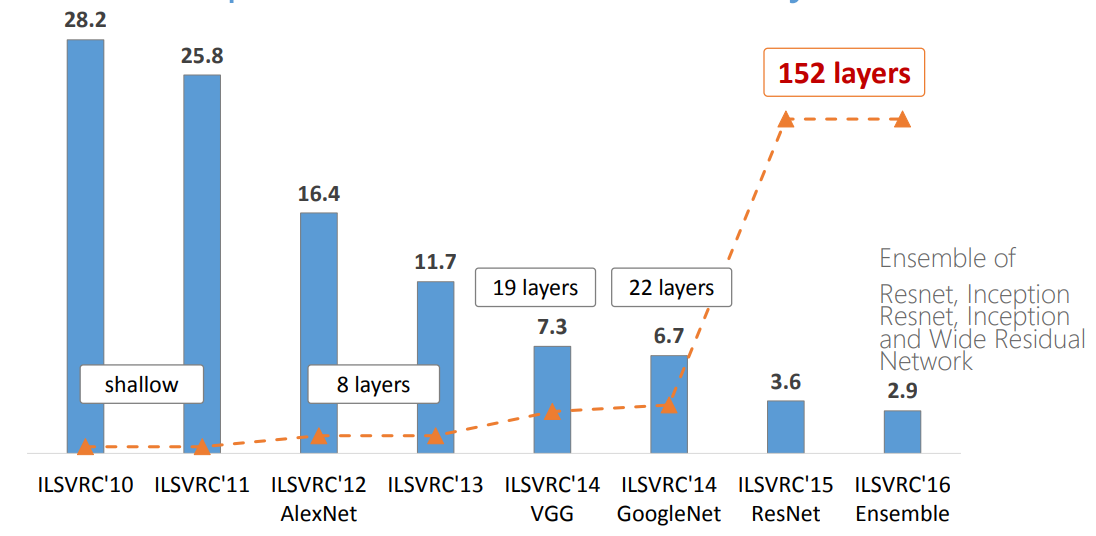
\includegraphics[width=\linewidth]{Screenshot.png}
		\subcaption{ImageNet Classification Top-5 error (\%)} 
	\end{subfigure}
	\begin{subfigure}[b]{0.475\textwidth}
		\centering
		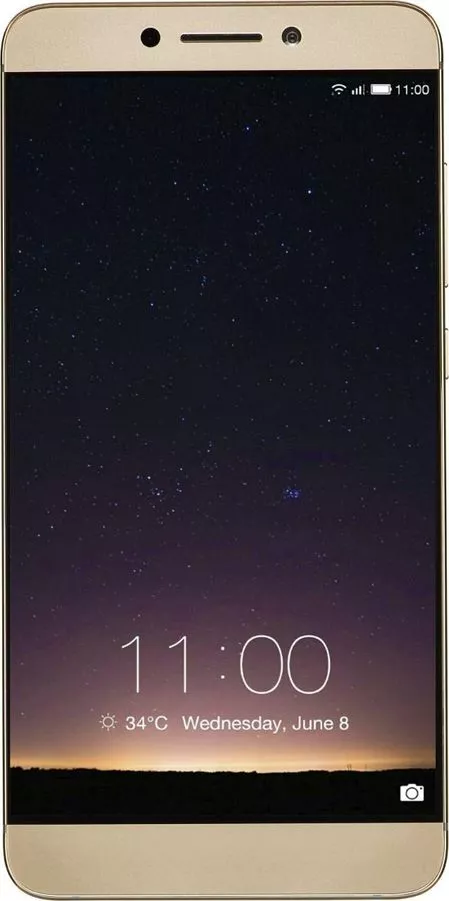
\includegraphics[width=0.2\linewidth]{leeco.png}
		\subcaption{Le 2 Smartphone}
	\end{subfigure}
	\caption{}
\end{figure}

CNNs have been the go to model for solving problems in Computer Vision. One such classical problem is the simultaneous recognition and localization of objects in an image (or video), also termed as Object detection. Object detection has achieved significant progress in the last few years, using deep convolutional networks. \cite{huang2017speed}. While accurate, these approaches have been too computationally intensive for embedded systems and, even with high-end hardware, too slow for real-time applications. In many real world applications such as robotics, self-driving car and augmented reality, the recognition tasks need to be carried out in a timely fashion on a computationally limited platform. This has led to recent interest in developing small and efficient neural networks such as Squeezenets, Mobilenets and Xnornet \cite{howard2017mobilenets,iandola2016squeezenet,rastegari2016xnor}, just to name a few. Here, we try to fine-tune a light, pre-trained object detection architecture on the KITTI \cite{geiger2012we} dataset and extract conclusions on its feasibility for autonomous driving or other driving assistance systems. This architecture is based on the Mobilenet feature head and the SSD detector. \cite{howard2017mobilenets,liu2016ssd}. After finetuning, the performance of the detector on the validation set is evaluated according to the VOC evaluation metrics \cite{everingham2010pascal}. We then deploy it on an Android device and asses the trade-offs between real time detection accuracy and speed while driving across university district. 
We will use LeEco's Le 2 smartphone as a platform to run the inferences using the trained model. It has a Qualcomm Snapdragon 652 chipset with 8 CPUs, four Cortex-A72 clocked at 1.8 Ghz each and another four Cortex-A53 clocked at 1.4 GHz each. It also consists of an Adreno 510 GPU and has a 3 GB RAM.

\section{Object Detection Pipeline}

As shown in Figure 2(a) all object detection algorithms consist of mainly three moving parts, the pre-processor, the feature extractor and the the proposal generator (or meta architecture).  The pre-processor takes in the raw images and performs image resizing, image pixel normalization and data augmentation operations, such as flips and random rotations, on it and makes it suitable to be fed into the feature extractor. The pre-processed image is then passed through the feature extractor, which is an off the shelf image classification network (VGG, Inception, Resnet, Inception Resnet, Googlenet or Mobilenet ) with its final few or all fully connected layers removed. It output a feature map, a mapping from high-dimensional, low level pixel space to low-dimensional high level feature space. This feature map is further passed through the detector Meta-architecture (or the meta architecture) to get bounding boxes and class probability for the image. The three main meta-architectures are the Single Shot Detection, R-FCN and the R-CNN. The meta architecture of R-FCN and Faster R-CNN consist of two different networks - a proposal generator to output bounding boxes and objectiveness and a box classifier to output class probability. Single Shot Detector modifies the proposal generator to directly output class probability instead of objectivetiness and is thus generally faster. YOLO and SSD Multibox detector(also known as SSD) are examples of single shot detection \cite{redmon2016you,liu2016ssd}. 

\begin{figure}[H]
	\centering
	\begin{subfigure}[b]{0.65\textwidth}
		\centering
		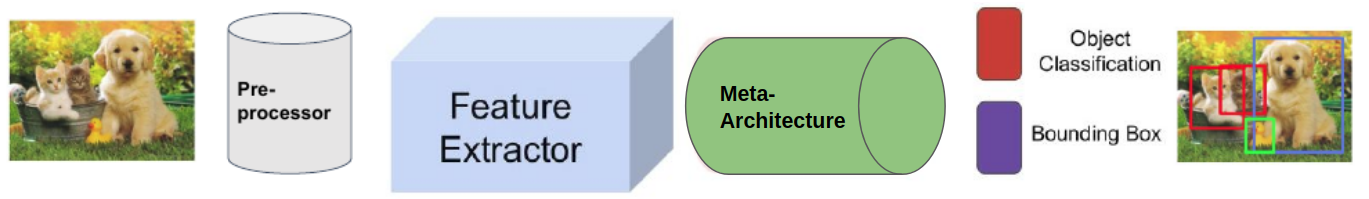
\includegraphics[width=\linewidth]{pipeline.png}
		\subcaption{Accuracy vs GPU Time for different extactor and meta-architecture combinations \cite{huang2017speed}} 
	\end{subfigure}
	\begin{subfigure}[b]{0.325\textwidth}
		\centering
		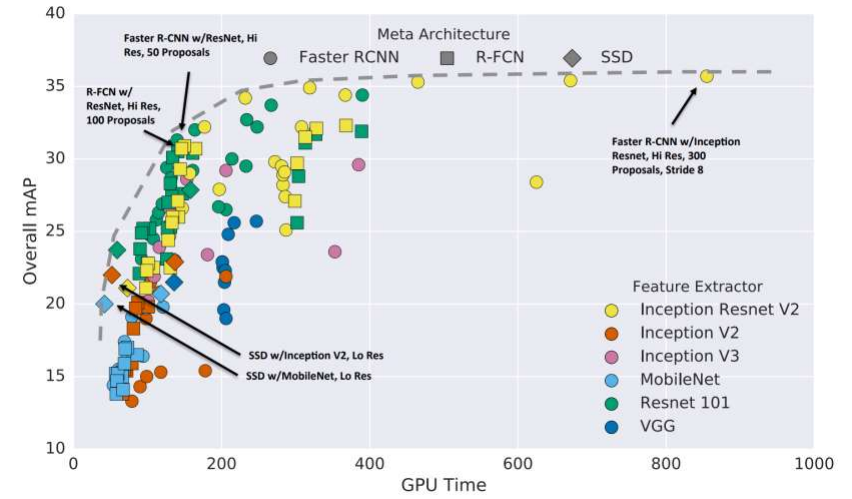
\includegraphics[width=\linewidth]{Screenshot1.png}
		\subcaption{Accuracy vs GPU time}
	\end{subfigure}
	\caption{}
\end{figure}

 A study at Google Research by Hunag et al\cite{huang2017speed} tried different combinations of feature extractor and meta-architectures and plotted the overall mAP value with GPU time, as can be seen in Figure 2(b). In general, Faster R-CNN is more accurate while R-FCN and SSD are faster. Faster R-CNN using Inception Resnet with 300 proposals gives the highest accuracy at 1 FPS. SSD on MobileNet has the highest mAP within the fastest models. This graph also helps us to locate some sweet spots with a good return in speed and cost tradeoff. R-FCN models using Residual Network strikes a good balance between accuracy and speed while Faster R-CNN with Resnet can attain similar performance if we restrict the number of proposals to 50.

\section{How Good is your Detection algorithm ?}

There are different metrics that exist for evaluating your algorithm. The three important ones are 
\begin{itemize}

\item \textbf{Mean Average Precision} This involves thresholding based on intersection of union score and then averaging over all class predictions. Higher the mAP the more accurate will be your detections.

\item \textbf{Inference time} This is the total time required to pre-process the image, pass it through the detector network and get a prediciton. 

\item \textbf{Memory usage} This refers to the model's cpu/gpu usage during prediction. Depending on the task and the resources available one should try to achieve a sweet-spot between the three.

\end{itemize}


Let us understand mAP in more detail as it would be used in further analysis.In order to calculate Mean Average Precision (mAP) in the context of Object Detection one must compute the Average Precision (AP) for each class, and then compute the mean across all classes. The key here is to compute the AP for each class, in general for computing Precision (P) and Recall (R) one must define what are: True Positives (TP), False Positives (FP), True Negative (TN) and False Negative (FN). In the setting of Object Detection of the Pascal VOC Challenge, these are the following:

\begin{equation}
P=\frac{TP}{TP+FP}, R=\frac{TP}{TP+FN}
\end{equation}

\begin{itemize}
\item \textbf{TP:} Those Bounding Boxes (BB) for which the intersection of union with ground truth boxes (GT) is more than 0.5
\item \textbf{FP:} BB for which the IoU with GT is below 0.5 and also the BB that has an IoU with a GT that has already been detected.
\item \textbf{TN:} there are no true negative, the image is expected to contain at least one object
\item \textbf{FN:} Those images where the method failed to produce a BB
\end{itemize}

Now once we have the precision recall values, we calculate AP (average precision) as average of 11 values of Precision at the points where Recall = $\left\{0, 0.1, 0.2, 0.3, 0.4, 0.5, 0.6, 0.7, 0.8, 0.9, 1\right\}$, i.e. $AP = \frac{1}{11} \sum_{R \in \left\{ 0, 0.1, ...., 1\right\}} P(R)$. Once we have the Average precision for each class, the mean precision is the weighted average of Average precision over all the classes.


\section{The Mobilenet-SSD Architecture}

The early network layers of the Mobilenet-SSD architecture is based on the mobilenet architecture \cite{howard2017mobilenets} which is a lightweight convolutional neural network which uses depthwise seperable convoltions to reduce the number of parameters and increase speed. Depthwise seperable convolution feactorize a standard convolution into a depthwise convoltuion and a $1 \times 1$ convolution called a pointwise convolution greatly reducing computation complexity. Figure 4 shows the SSD based detector with VGG-16 base network, a Mobilenet-SSD is similar to this architecture where the VGG-16 base network is replaced by Mobilenet.
 The SSD meta-arachitecture adds convolutional feature layers to the end of the truncated base network. These layers progressively decrease in size allowing for predictions at multiple scale.  We apply on top of each convolutional feature map (output of SSD's convolutional feature layer) a set of filters that predict detections for different aspect ratios
and class categories

\begin{figure}[H]
	\centering
	\begin{subfigure}[b]{0.475\textwidth}
		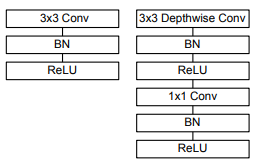
\includegraphics[width=\linewidth]{depthwise.png}
		\subcaption{Depthwise Seperable Convolution}
	\end{subfigure}
	\begin{subfigure}[b]{0.475\textwidth}
		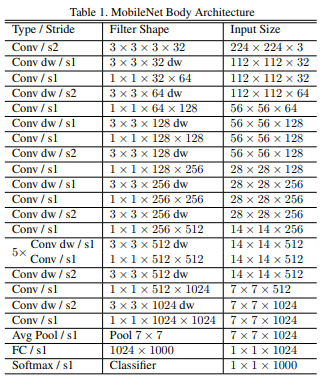
\includegraphics[width=0.75\linewidth]{mobilenet.png}
		\subcaption{Mobilenet Architecture}
	\end{subfigure}
	\caption{}
\end{figure}

\begin{figure}[H]
	\centering
	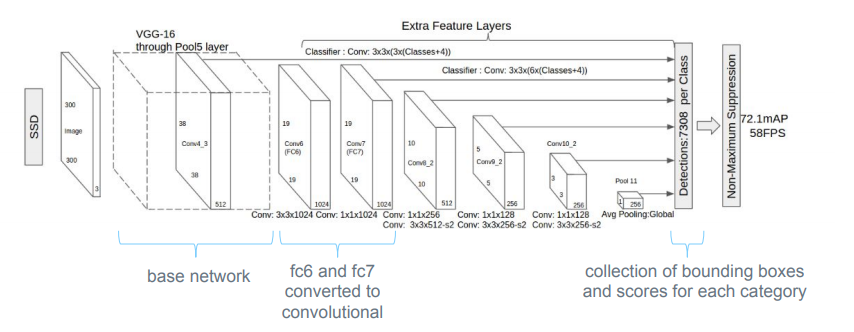
\includegraphics[width=\linewidth]{ssd.png}
	\caption{Single Shot Multibox detector (SSD)}
\end{figure}




\section{KITTI Dataset}

KITTI Vision Benchmark Suite datasets \cite{geiger2012we} are captured
from driving sessions around the city of Karlsruhe (Germany),
in rural areas and on highways. It consist of 7481 training images, each with a resolution of $1240\times 375$ pixels. Since the testing images in this dataset aren't labelled 80\% of the training images are used as training data and the rest 20\% is used as validation data. The dataset consist of 11 annotated classes out of which the main classes present are: cars, with
28.742 samples, followed by pedestrians, with 4.487 samples and cyclists, with 1.627 samples. We use 5 classes for finetuning the Mobilenet-SSD model - car, pedestrian, cyclist, truck and van.
\begin{figure}[H]
	\centering
	\begin{subfigure}[b]{0.475\textwidth}
		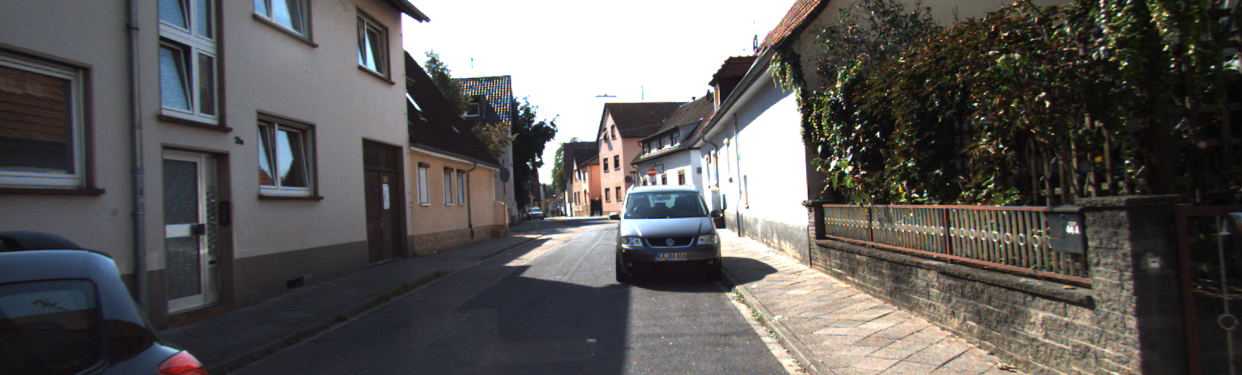
\includegraphics[width=\linewidth]{000003.png}
	\end{subfigure}
	\begin{subfigure}[b]{0.475\textwidth}
		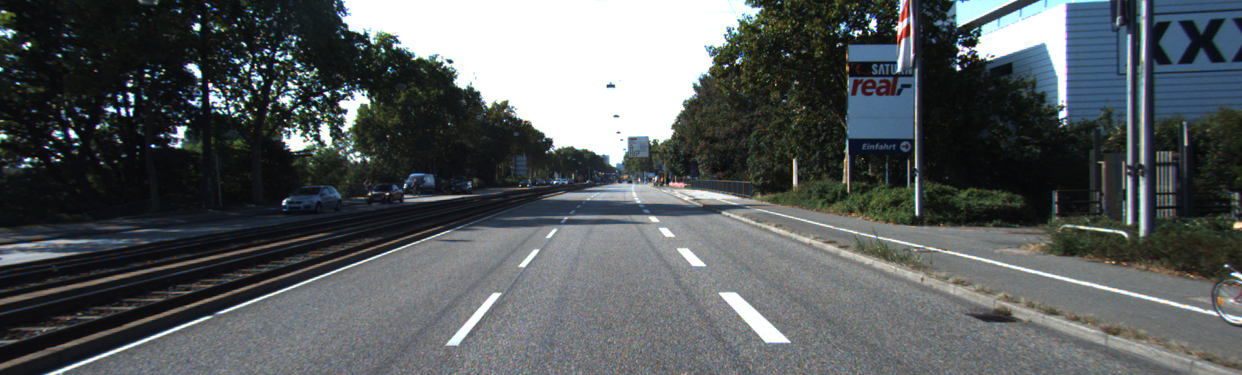
\includegraphics[width=\linewidth]{000004.png}
	\end{subfigure}
	\\
	\begin{subfigure}[b]{0.475\textwidth}
		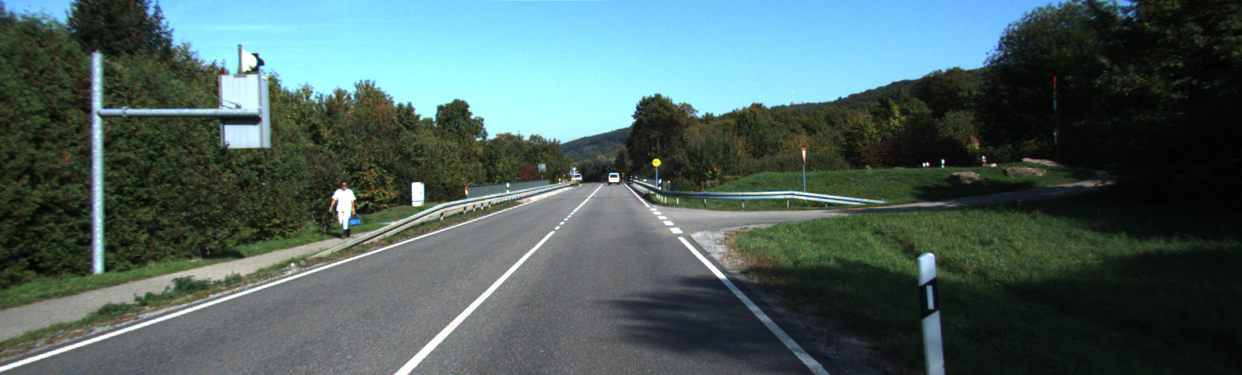
\includegraphics[width=\linewidth]{000005.png}
	\end{subfigure}
	\begin{subfigure}[b]{0.475\textwidth}
		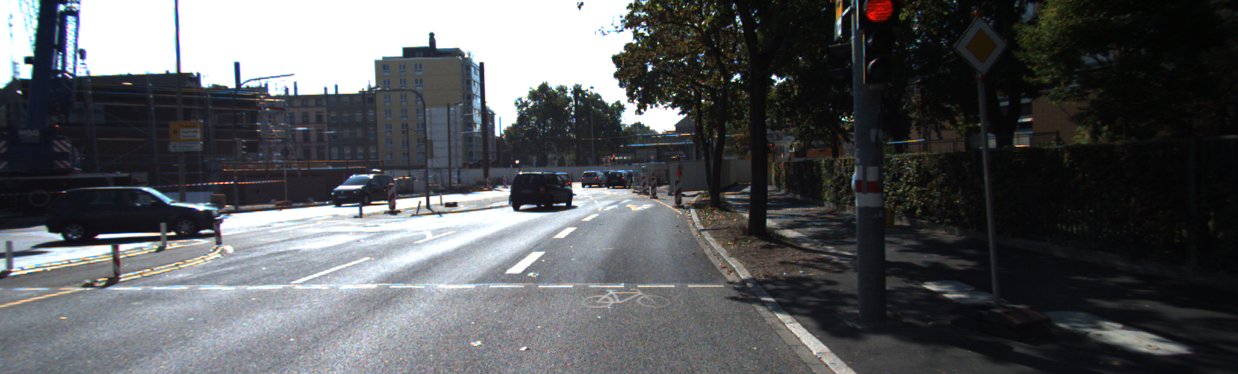
\includegraphics[width=\linewidth]{000006.png}
	\end{subfigure}
	\caption{Images from the KITTI dataset}
\end{figure}

\section{Transfer Learning}

We finetune the MobileNet SSD Model pre-trained for the coco dataset (called \code{ssd\_mobilenet\_v1\_coco} and downloaded from Tensorflow detection model zoo). Horizontal flipping which involves mirroring the image and random cropping operations are applied to the input training images to augment the dataset. The entire network is trained using a batch-size of 32 images and a momentum based RMSprop optimizer. The learning rate of the optimizer is initially set to 0.004 and allowed to exponentially decay with a decay factor of 0.95 and with 800720 as the decay steps. The other hyper-parameter values used are, momentum optimizer value=0.9, decay=0.9 and epsilon=1.0 .  

\subsection{Loss function}

The overall loss function as proposed in \cite{liu2016ssd} is calculated as the weighted sum of localization loss and classification loss (also known as confidence loss). Localization loss is a measure of how close are the bounding boxes the model created to the ground truth boxes. The classification(or confidence loss) is a measure of how accurately does the model predict the class of each object. Here, we use use a weighted sigmoid classification loss and a weighted smooth L1 localization loss. These two losses are equally weighted when calculating the final total loss. Below we have summarized the nomencalure for defining losses

$\bm{L}$: Total loss, $\bm{L_{conf}}$: Confidence (or Classification) loss, $\bm{L_{loc}}$: Localization loss, \textbf{\textit{l}}: predicted box, \textbf{\textit{g}}: ground truth box, \textbf{\textit{d}}: default box, \textbf{\textit{N}}: number of default boxes, \textbf{\textit(cx, cy)}:center of the default bounding box, \textbf{\textit{w}}: width of the bounding box, \textbf{\textit{h}}: height of the bounding box.

\begin{equation}
L(x,c,l,g)=\frac{1}{N}(L_{conf}(x,c)+L_{loc}(x,l,g))
\end{equation}

\subsubsection{Localization loss}

The localization loss is calculated only on positive boxes (ones with a matched ground truth). It calculates the difference between the correct and predicted offsets to center point coordinates, and the correct and predicted scales to the widths and heights. And smooth the absolute differences.

\begin{equation}
L_{loc}(x,l,g)=\sum_{i \in Pos}\sum_{m \in \left\{ cx, cy, w,h\right\}}x_{i,j}^{k}\text{smooth}_{L_{1}}(l_{i}^{m}-\hat{g}_{j}^{m})
\end{equation}

\begin{equation}
\hat{g}_{j}^{cx}=\frac{(g_{j}^{cx}-d_{i}^{cx})}{d_{i}^{w}}, \hat{g}_{j}^{cy}=\frac{(g_{j}^{cy}-d_{i}^{cy})}{d_{i}^{h}}, \hat{g}_{j}^{w} =\text{log}(\frac{g_{j}}{d_{i}^{w}}), \hat{g}_{j}^{h}=\text{log}(\frac{g_{j}^{h}}{d_{i}^{h}}) 
\end{equation}

\[
    \text{smooth}_{L_{1}}(x)= 
\begin{cases}
    0.5x^{2},& \text{if } |x| < 1\\
    |x|-0.5,              & \text{otherwise}
\end{cases}
\]

where, $x_{i,j}^{p}=\left\{ 1,0\right\}$ is the indicator function for matching the $i-$th default box to the $j-$th ground truth box of category $p$

\subsubsection{Classification loss(or Confidence loss)}

The confidence loss is the softmax loss over multiple classes confidences (c).

\begin{equation}
L_{conf}(x,c)=-\sum_{i \in Pos}^{N}x_{i,j}^{p}log(\hat{c}_{i}^{p})-\sum_{i \in Neg}log(\hat{c}_{i}^{0})
\end{equation}

where $\hat{c}_{i}^{p}=\frac{e^{c_{i}^{p}}}{\sum_{p}e^{c_{i}^{p}}}$

\subsection{Training}

For training an object detection pipeline we need both positive and negative examples.Here, 
Online Hard example algorithm \cite{shrivastava2016training} is used for training. It reduces computation by running hard example mining hand to hand with the regular optimization cycle. In general, to pick a subset of negatives, we first train our network for couple of iterations, then it is run all along our negative instances before we pick the ones with the greater loss values. However, it is very computationally toilsome since we have possibly millions of images to process, and sub-optimal for the optimization process since we freeze our network while picking the hard instances. That is, you assume here all hard negatives you pick are useful for all the next iterations until the next selection. Which is an imperfect assumption especially for large datasets. Online means in this regard. OHEM solves these two aforementioned problems by performing hard example selection batch-wise. Given a batch sized $k$, it performs regular forward propagation and computes per instance losses. Then, it finds $m < k$ hard examples in the batch with high loss values and it only back-propagates the loss computed over the  selected instances.


\section{Results and Discussions}

\begin{table}[ht]
\begin{minipage}[b]{0.55\linewidth}
\centering
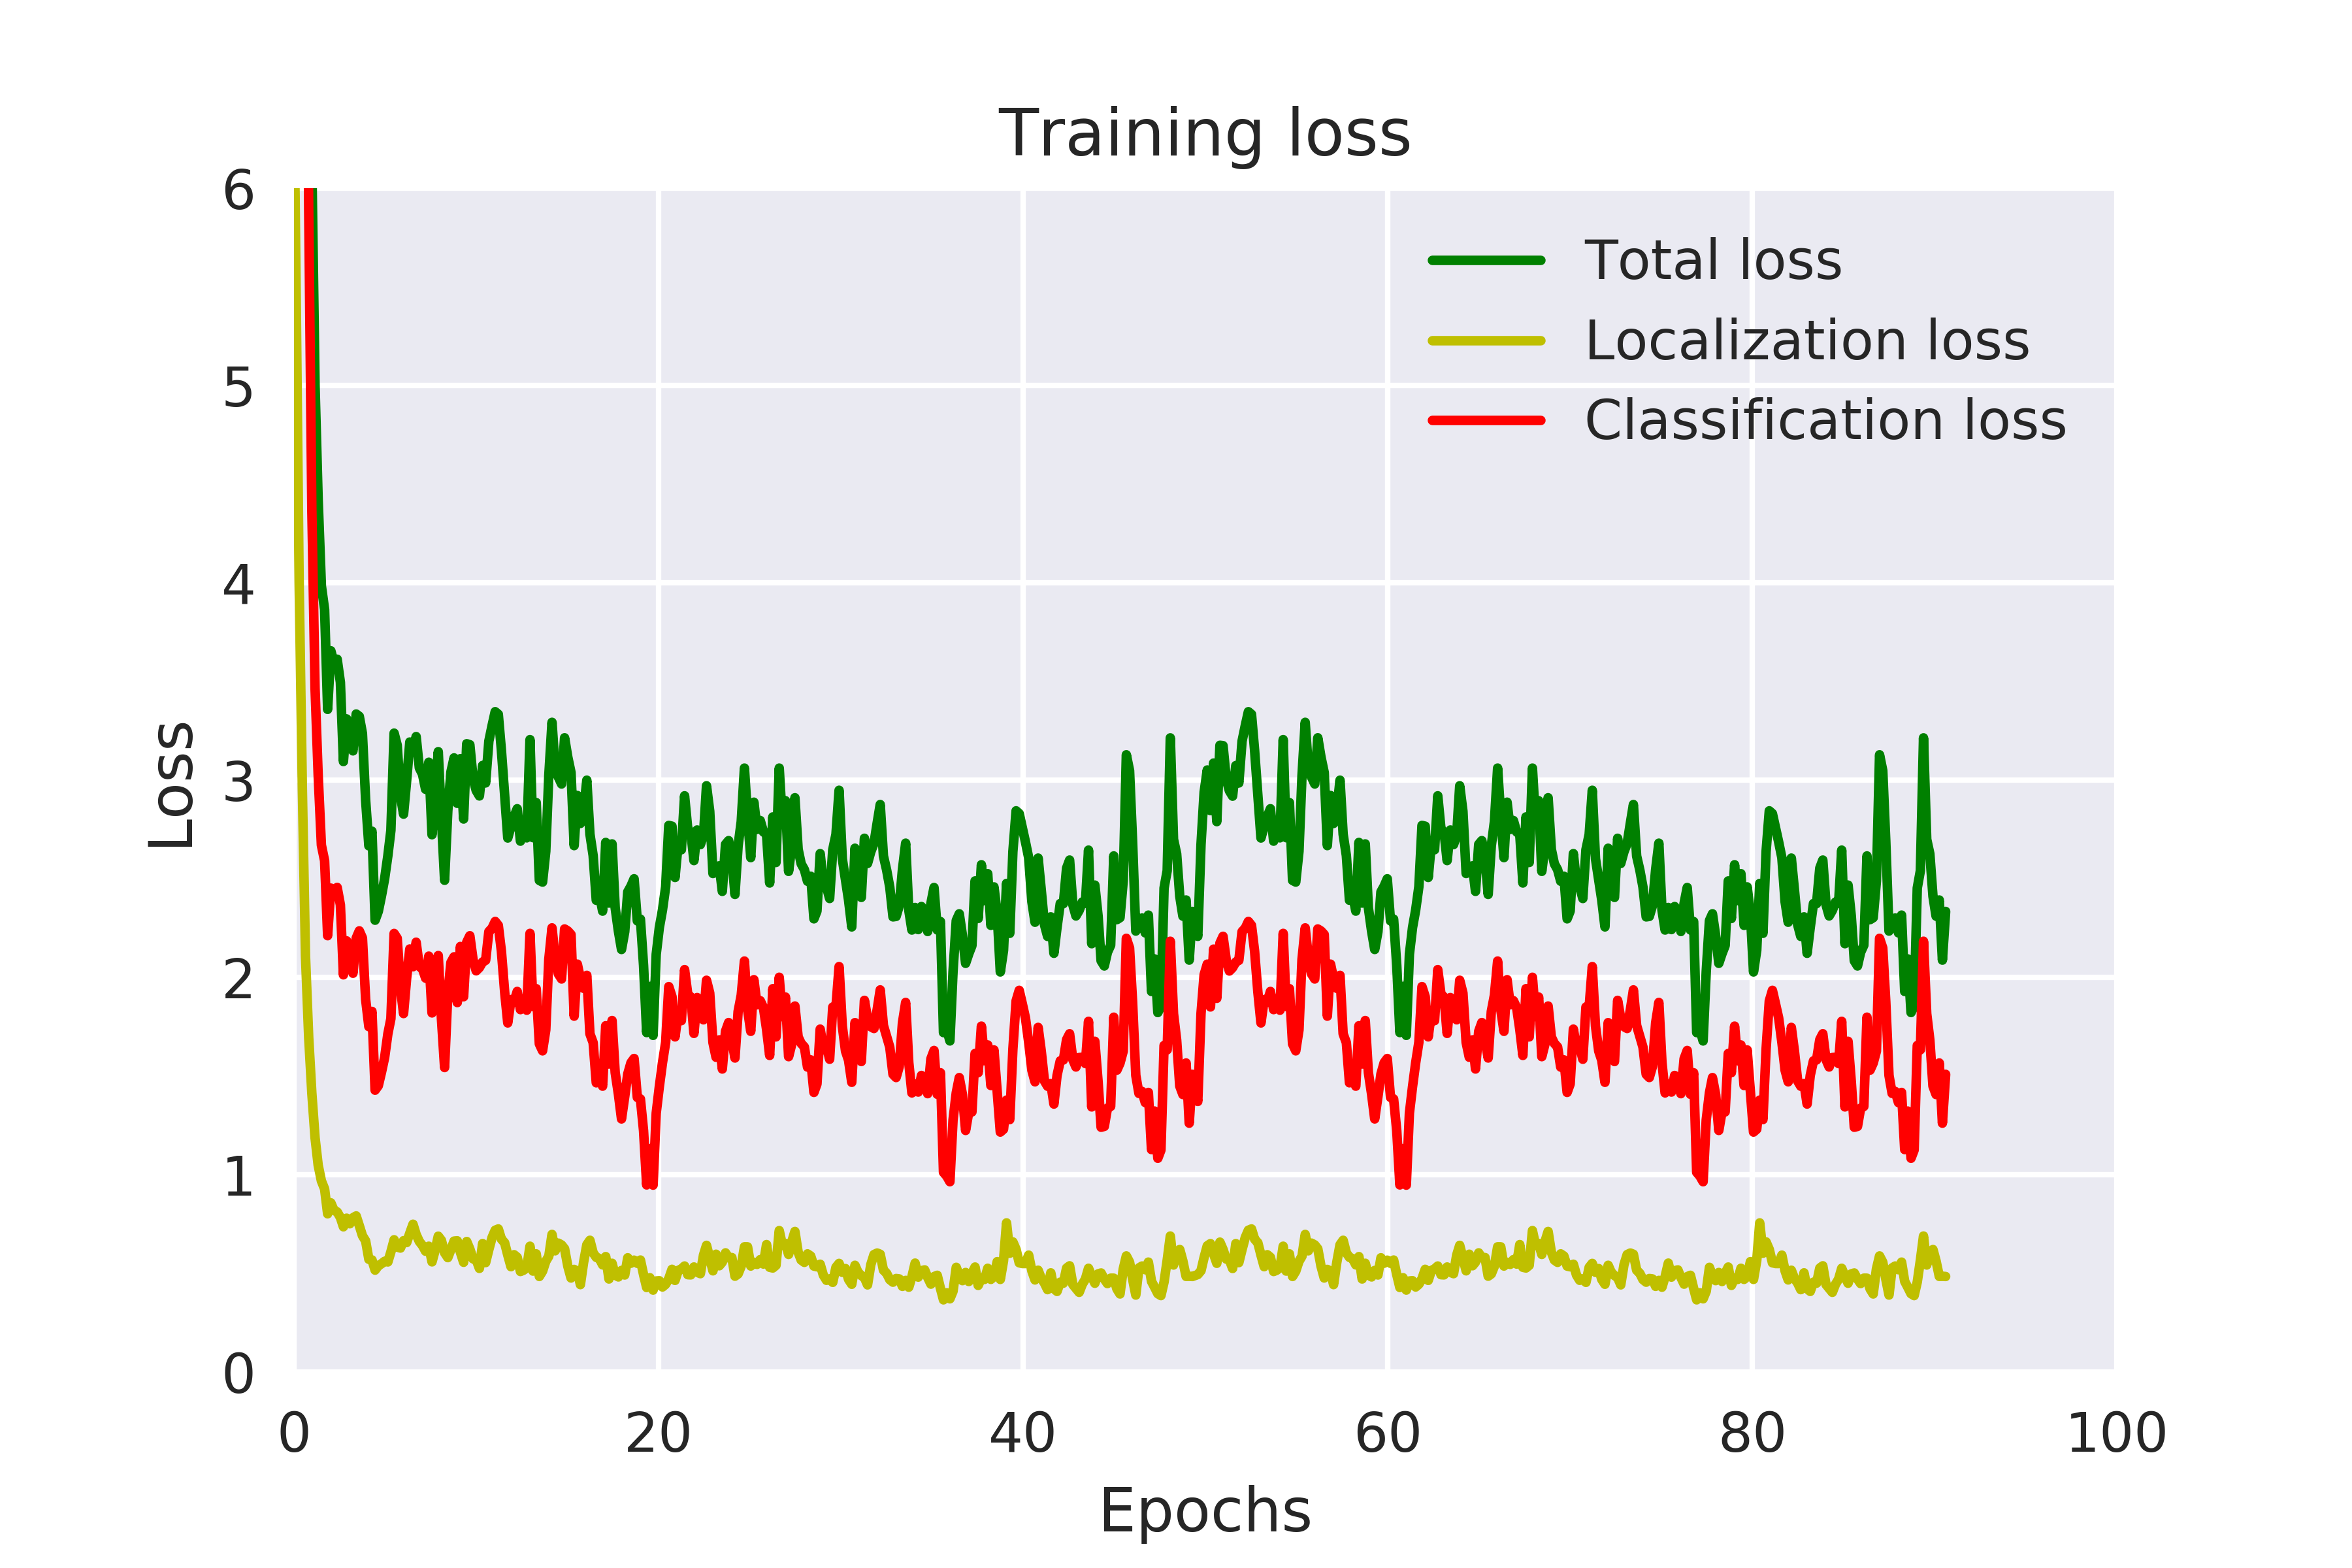
\includegraphics[width=80mm]{loss.png}
\captionof{figure}{2-D scatterplot of the Student Database}
\label{fig:image}
\end{minipage}
\begin{minipage}[b]{0.25\linewidth}
\centering
\begin{tabular}{ | l | r | }
    \hline
    Category & Average Precision \\ \hline \hline
    Car & 0.76\\ \hline
    Pedestrian & 0.72  \\ \hline
    Cyclist & 0.38\\ \hline
    Truck & 0.51\\ \hline
    Van & 0.35\\ \hline
    \textbf{Overall} & 0.544 \\ \hline
   \end{tabular}
    \caption{Average Precision on the Validation set}
    \label{table:student}
\end{minipage}\hfill
\end{table}

The training was done on UW's Hyak cluster using a P100 GPU. Figure 6 shows how the three losses, total loss, classification loss and localization loss evolves with the number of epochs. These values have been exponentially smoothed out with a smoothing factor of 0.6. The trained model is then evaluated on the validation set we had set aside consisting of 20 \% of KITTI training images. mAP scores are calculated on this validation set using VOC Evaluation criteria we have previously explained in section 3.
As it can be seen from the mAP scores in Table 1 or from the example predictions on validation set images in Figure 7, the network is way better in detecting cars and pedestrians compared to other classes. The reason might be that the number of instances of car and pedestrian class is the maximum in the dataset , much higher than the other classes, with cyclist class coming third. Thus the network has enough examples to learn the corresponding features of the car and pedestrian really well. Also, we changed our image resolution from $1240 \times 375$ to $300 \times 300$ before feeding it to the Mobilenet feature extractor (This is because the Mobilenet we used was designed to work on $300 \times 300$ images). This naive trick is probably not the best way to go about resizing the images and what we could do in the future is maintain the aspect ratio while resizing and then pad the edges to get a $300 \times 300$ image.
\begin{figure}
	\centering
	\begin{subfigure}[b]{0.45\textwidth}
		\centering
		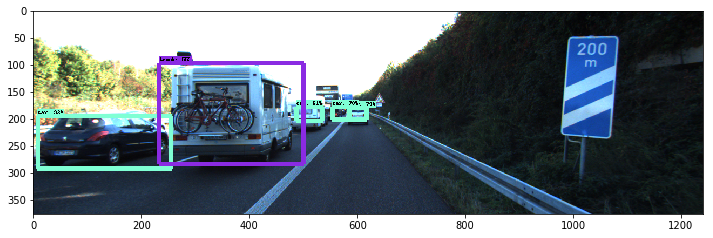
\includegraphics[width=\linewidth]{val_1.png}
	\end{subfigure}
	\begin{subfigure}[b]{0.45\textwidth}
		\centering
		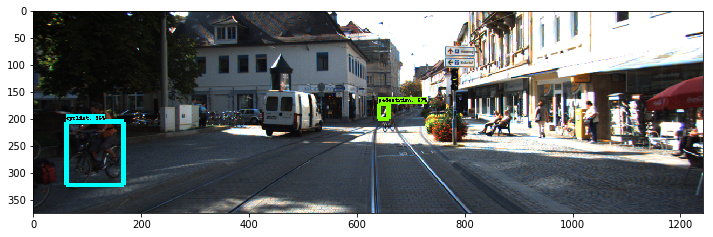
\includegraphics[width=\linewidth]{val_2.png}
	\end{subfigure}
	\\
	\begin{subfigure}[b]{0.45\textwidth}
		\centering
		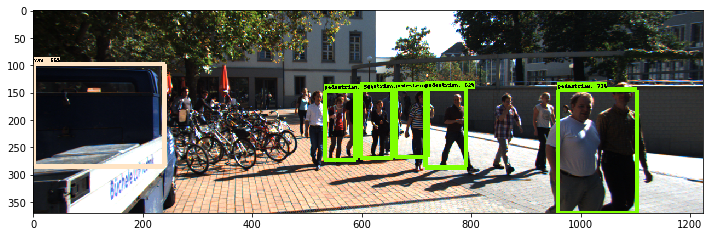
\includegraphics[width=\linewidth]{val_3.png}
	\end{subfigure}
	\begin{subfigure}[b]{0.45\textwidth}
		\centering
		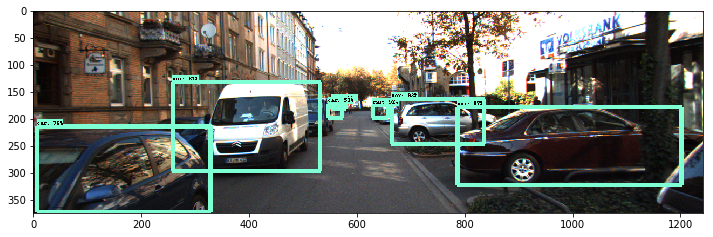
\includegraphics[width=\linewidth]{val_4.png}
	\end{subfigure}
	\caption{Example predictions from validation set}
\end{figure}

\subsection{Android Implementation and Benchmarking}

Leeco's Le 2 model was used to test the android implementation of the trained model. We make use of the "Tensorflow Android Inference Interface" which provides the ability to load a tensorflow graph, set up the inputs and run the model to calculate particular outputs. First, the trained model is freezed into a protobuf file. This protobuf file is further optimized for inferece-only purposes by removing parts that are only needed during training. To get the entire model working on our android device we need the tensorflow libraries for Android (Tensorflow Android Inference Interface), create an Android App that has access to live camera stream and configure it to use these libraries, and then invoke the tensorflow model inside the app. After getting the entire set-up working we drove around University district to test how to asses its performance. Figure 8 and 9 consist of three different scenarios, one in each row - "stopping at an intersection", "following a cyclist", "taking a trun", "driving past a truck". The images in each row have a 1 second time difference with it's neighbouring frame. As it can be clearly seen that the setup isn't exactly real time and for most moving objects the bounding boxes seem to follow the object with a delay of about 1-2 seconds even when the car is stationary. The entire video can be accessed \href{https://drive.google.com/drive/folders/1nKVbr_vOX3ATzaXllUpJjq_BlYVBL-1D?usp=sharing}{here}.

\begin{figure}[H]
	\centering
	\begin{subfigure}[b]{0.15\textwidth}
		\centering
		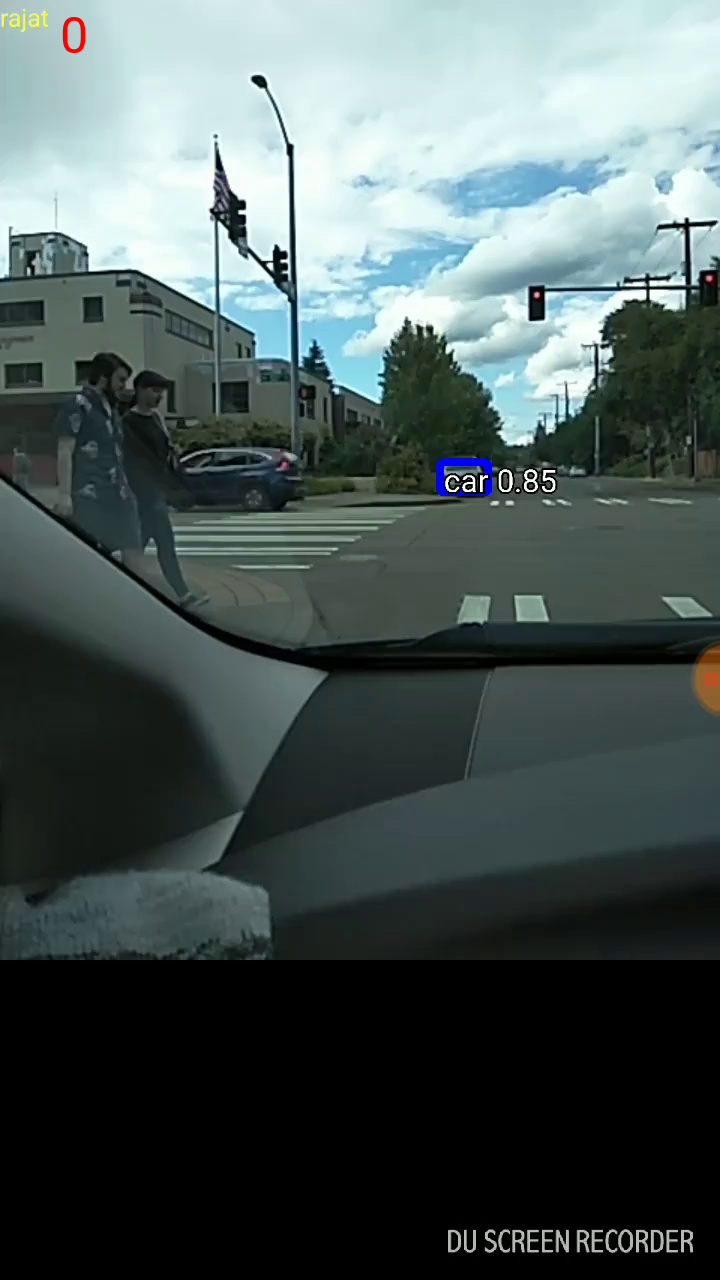
\includegraphics[width=\linewidth]{results/result_0.png}
	\end{subfigure}
	\begin{subfigure}[b]{0.15\textwidth}
		\centering
		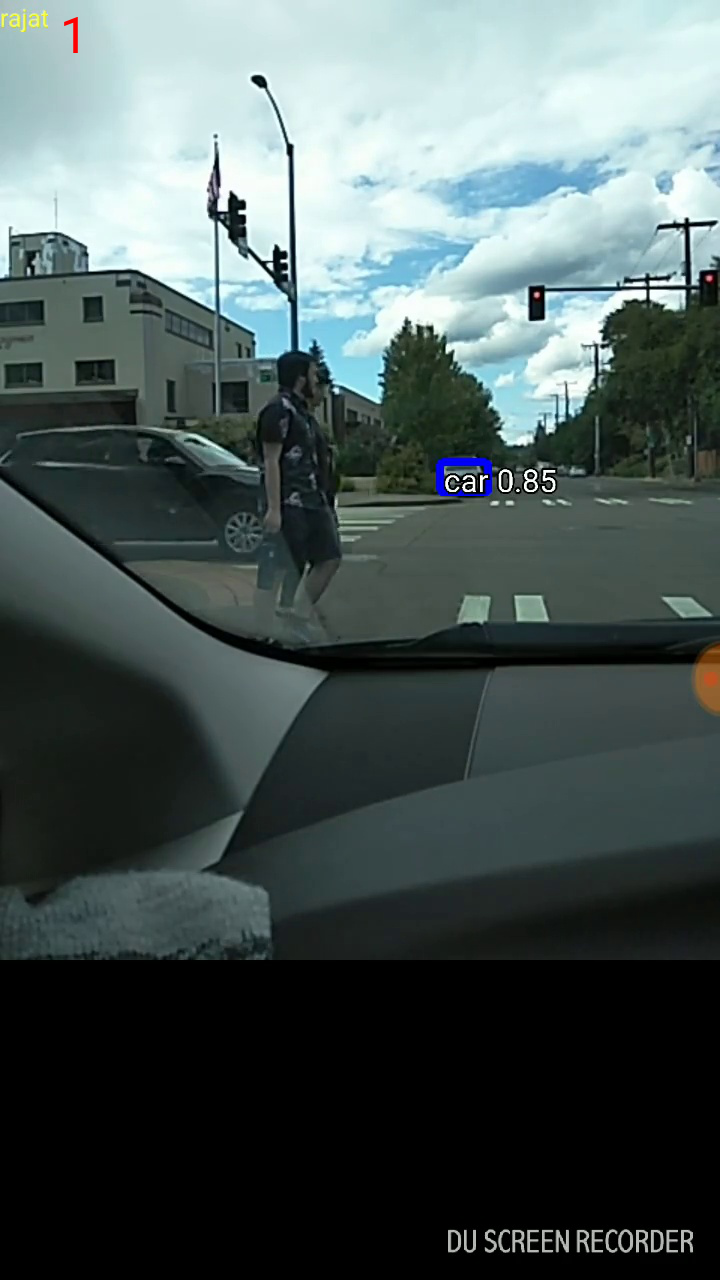
\includegraphics[width=\linewidth]{results/result_40.png}
	\end{subfigure}
	\begin{subfigure}[b]{0.15\textwidth}
		\centering
		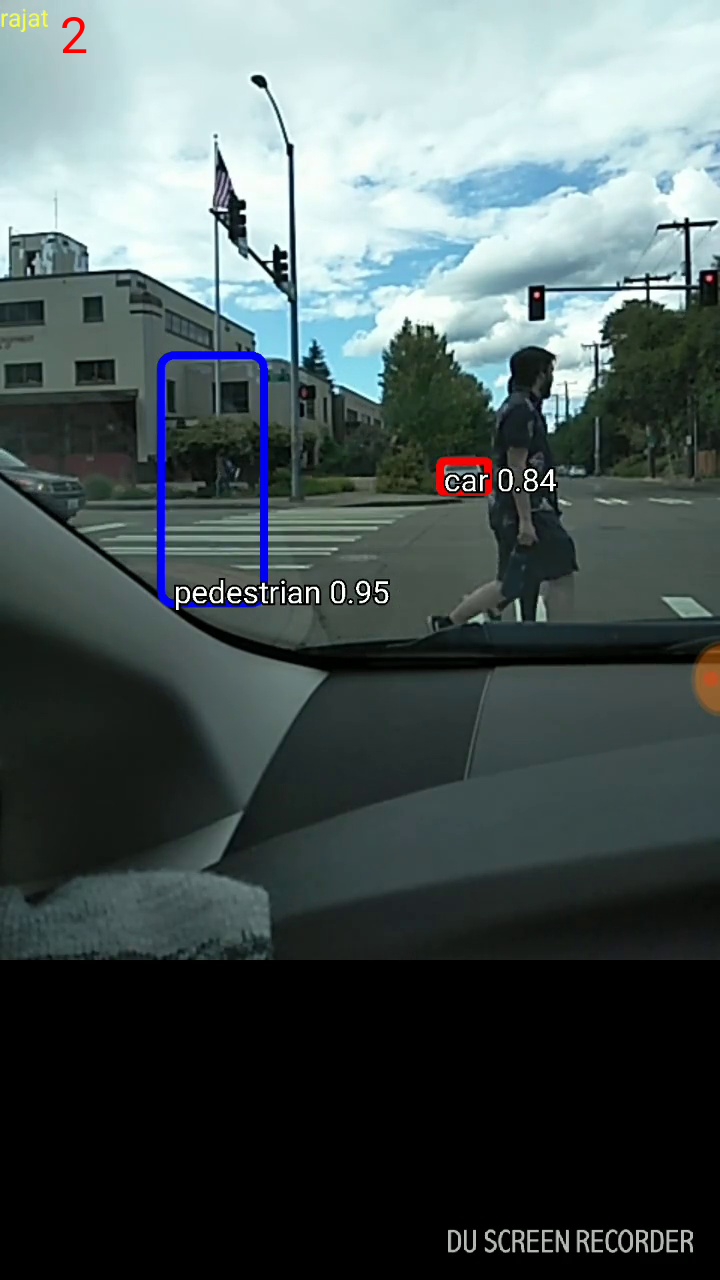
\includegraphics[width=\linewidth]{results/result_80.png}
	\end{subfigure}
	\begin{subfigure}[b]{0.15\textwidth}
		\centering
		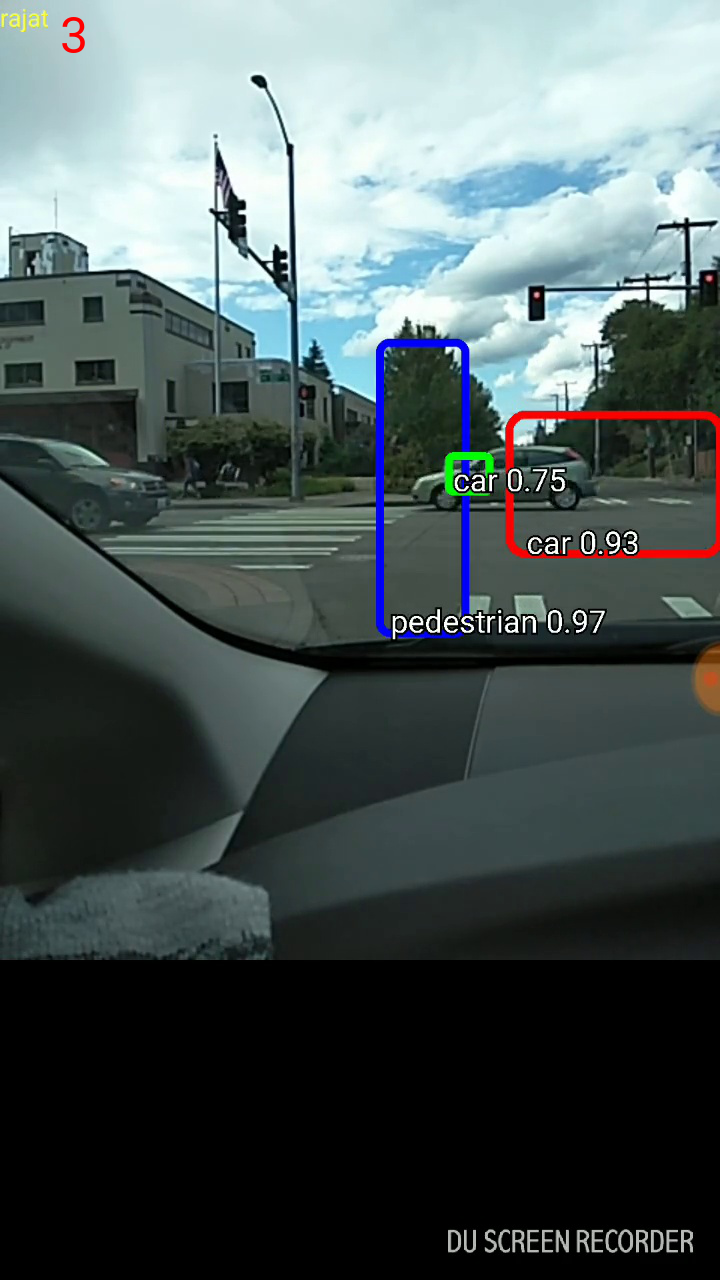
\includegraphics[width=\linewidth]{results/result_120.png}
	\end{subfigure}
	\begin{subfigure}[b]{0.15\textwidth}
		\centering
		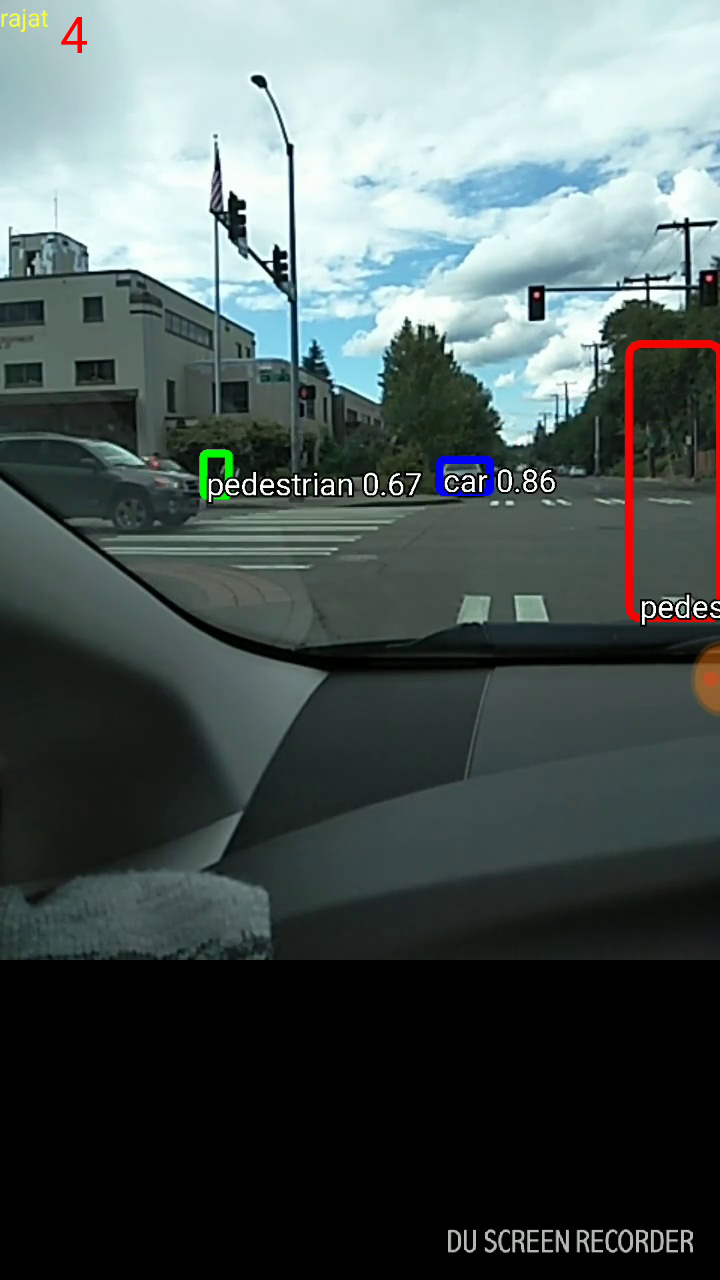
\includegraphics[width=\linewidth]{results/result_160.png}
	\end{subfigure}
	\begin{subfigure}[b]{0.15\textwidth}
		\centering
		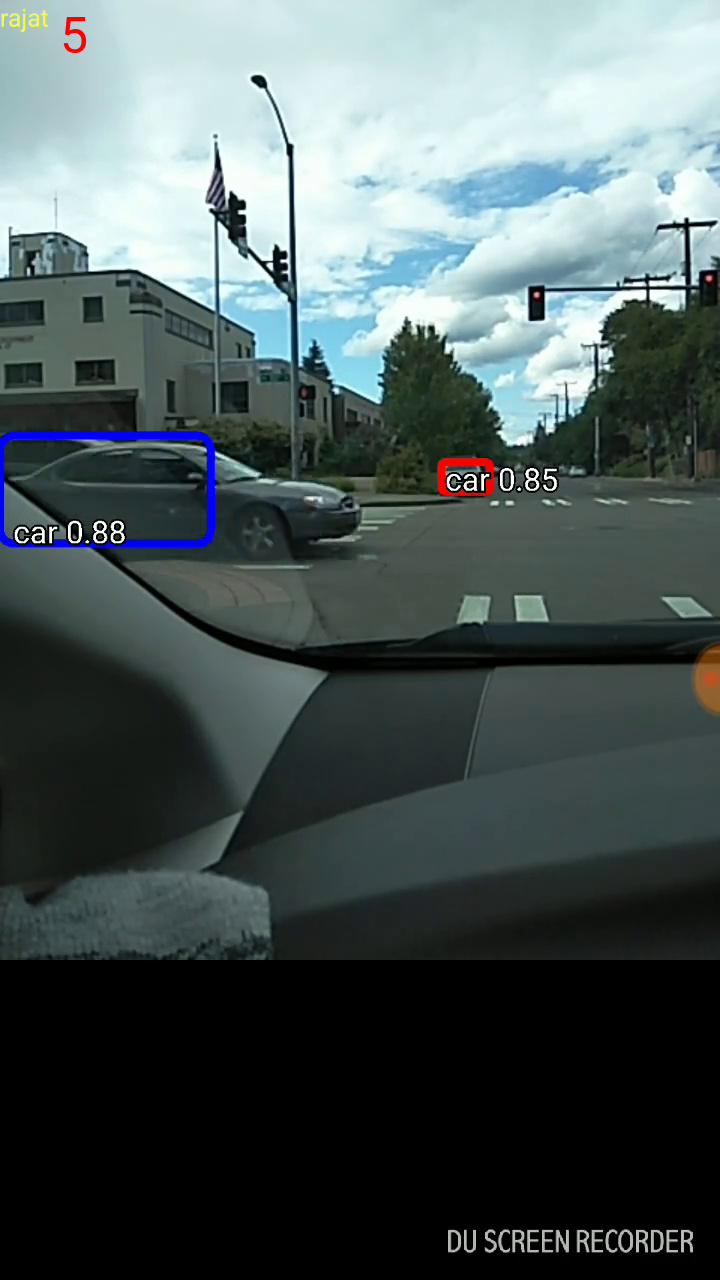
\includegraphics[width=\linewidth]{results/result_200.png}
	\end{subfigure}

		\begin{subfigure}[b]{0.15\textwidth}
		\centering
		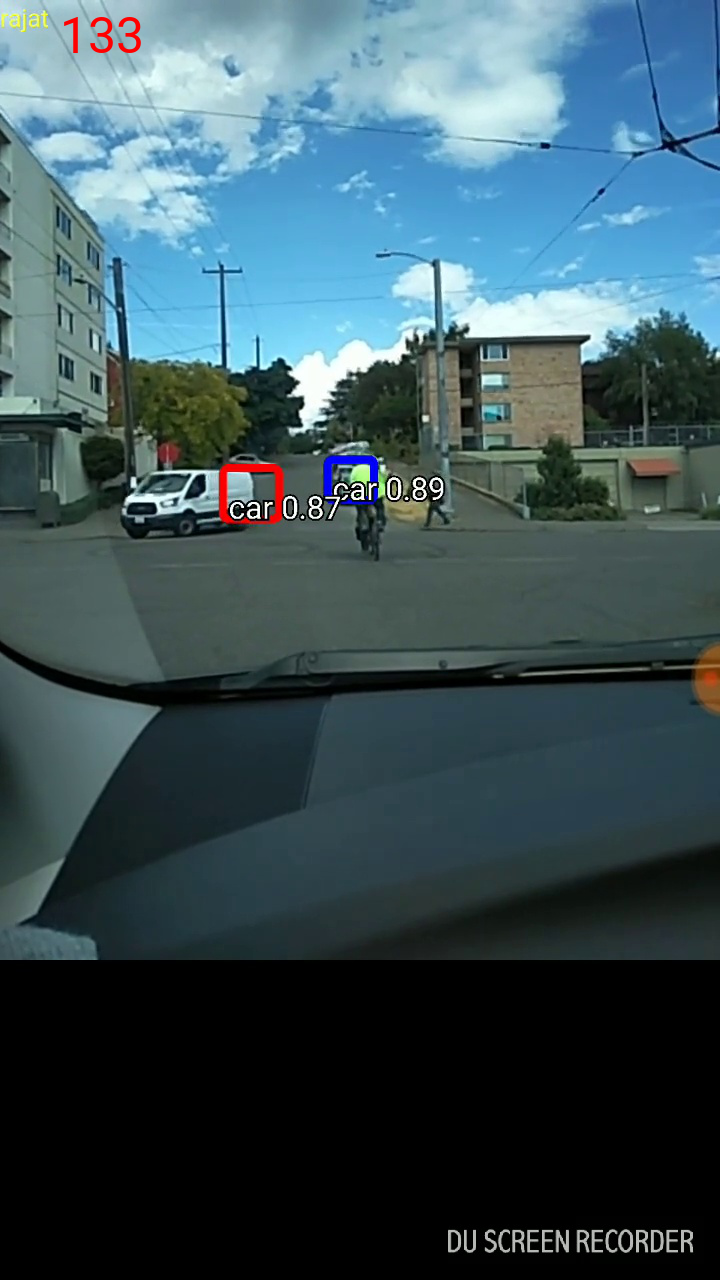
\includegraphics[width=\linewidth]{results/result_5320.png}
	\end{subfigure}
	\begin{subfigure}[b]{0.15\textwidth}
		\centering
		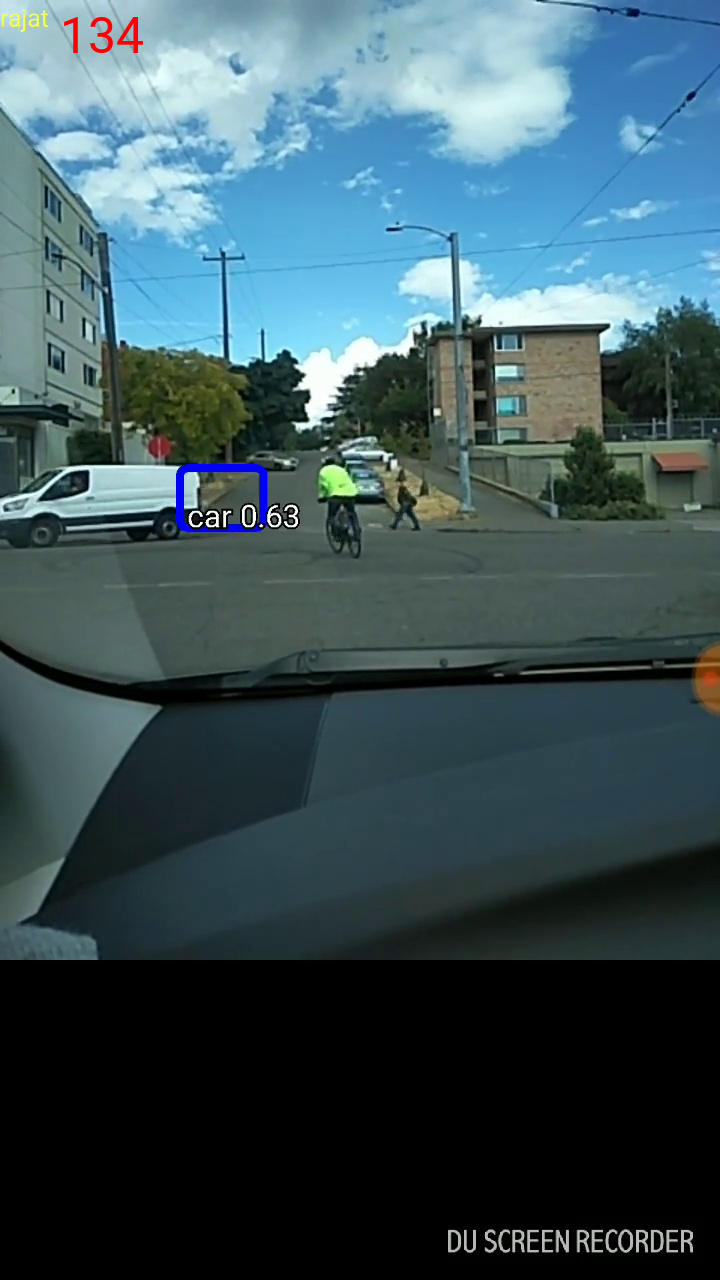
\includegraphics[width=\linewidth]{results/result_5360.png}
	\end{subfigure}
	\begin{subfigure}[b]{0.15\textwidth}
		\centering
		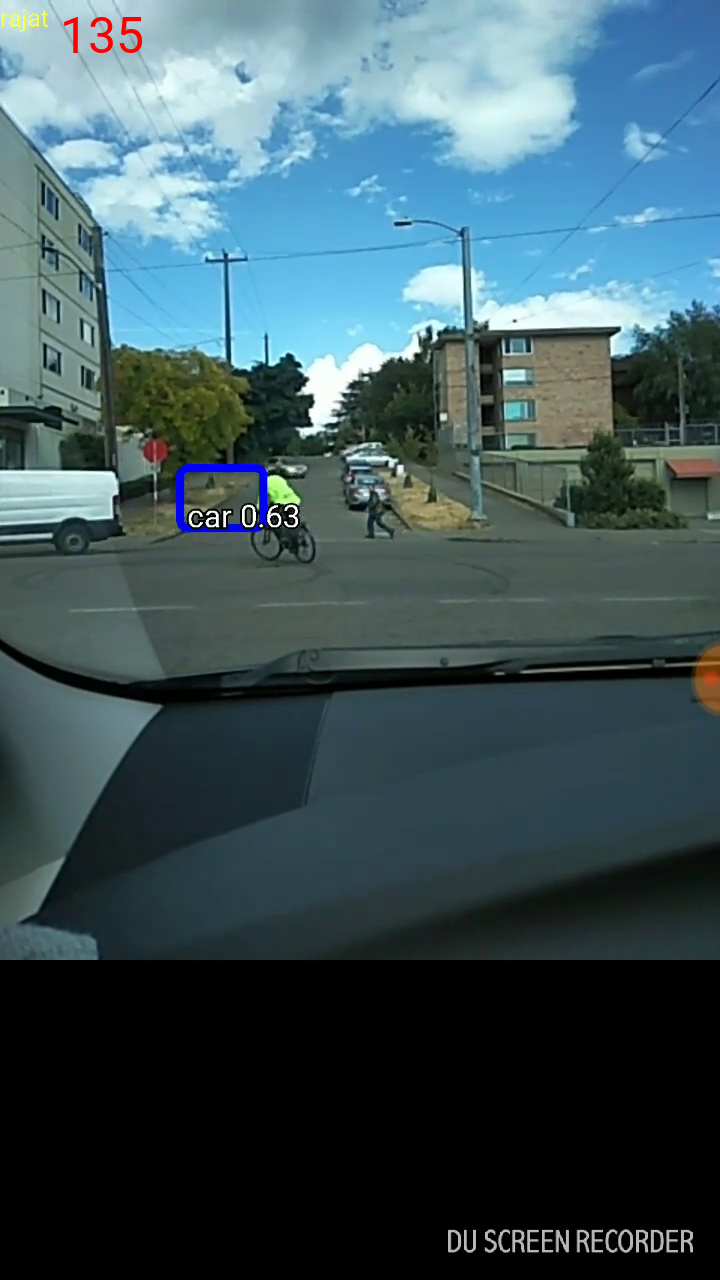
\includegraphics[width=\linewidth]{results/result_5400.png}
	\end{subfigure}
	\begin{subfigure}[b]{0.15\textwidth}
		\centering
		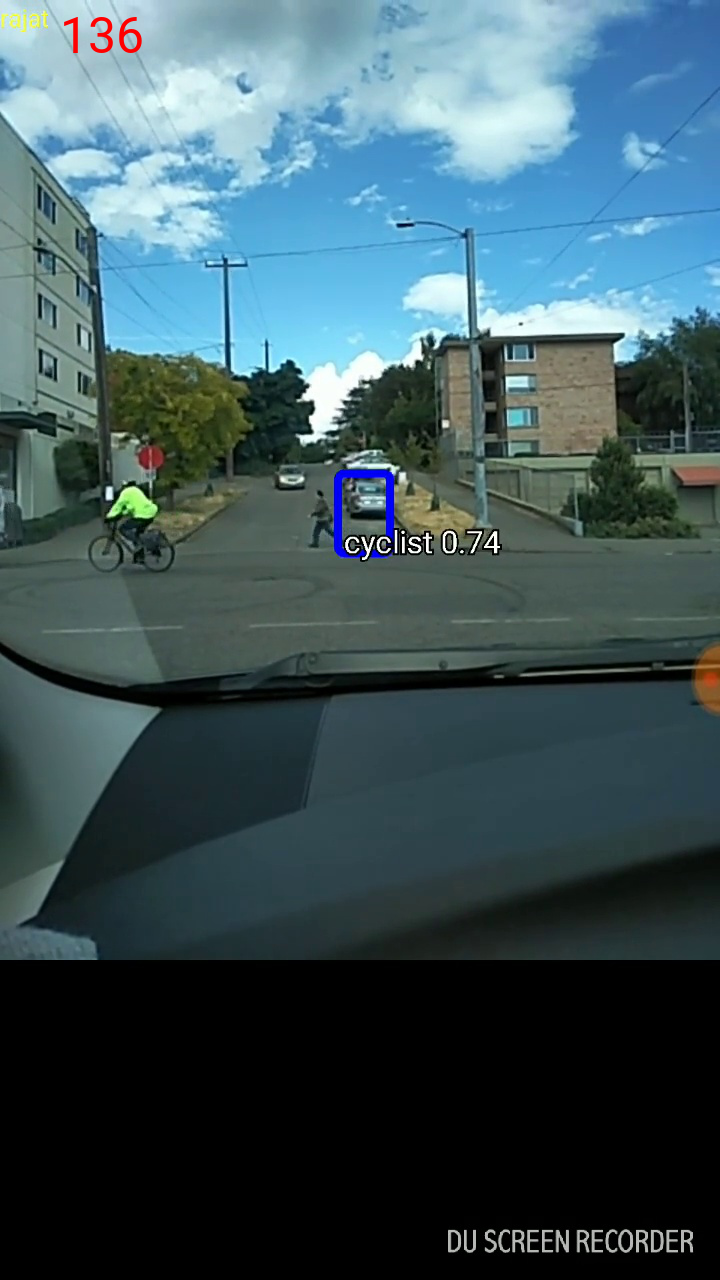
\includegraphics[width=\linewidth]{results/result_5440.png}
	\end{subfigure}
	\begin{subfigure}[b]{0.15\textwidth}
		\centering
		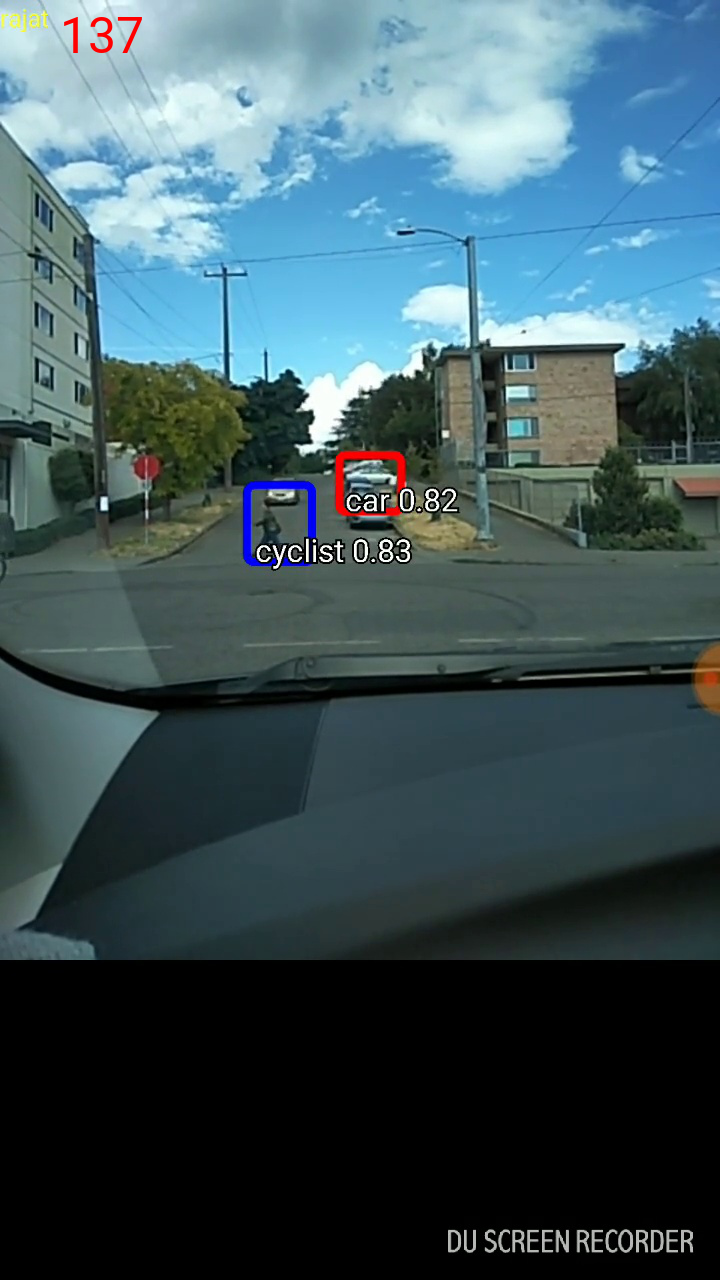
\includegraphics[width=\linewidth]{results/result_5480.png}
	\end{subfigure}
	\begin{subfigure}[b]{0.15\textwidth}
		\centering
		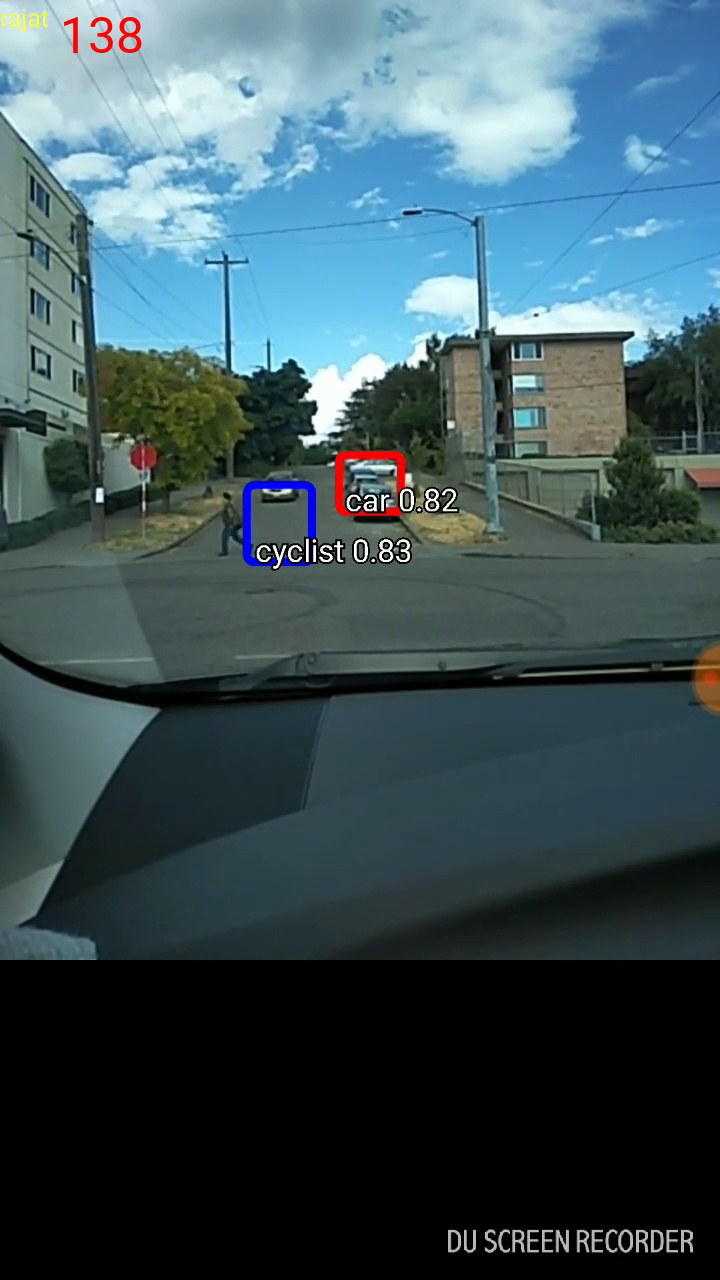
\includegraphics[width=\linewidth]{results/result_5520.png}
	\end{subfigure}

	\caption{(a) Stopping at an intersection (b) Following a cyclist}
\end{figure}

\begin{figure}[H]
\centering
		\begin{subfigure}[b]{0.15\textwidth}
		\centering
		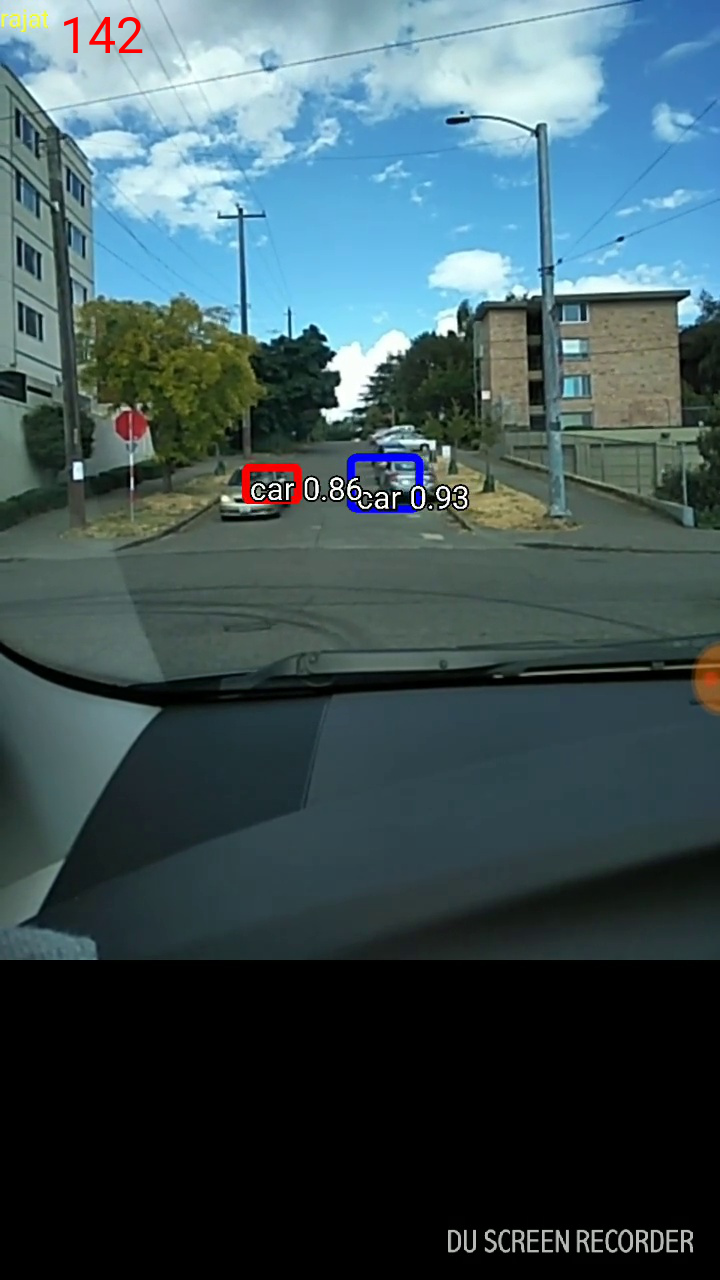
\includegraphics[width=\linewidth]{results/result_5680.png}
	\end{subfigure}
	\begin{subfigure}[b]{0.15\textwidth}
		\centering
		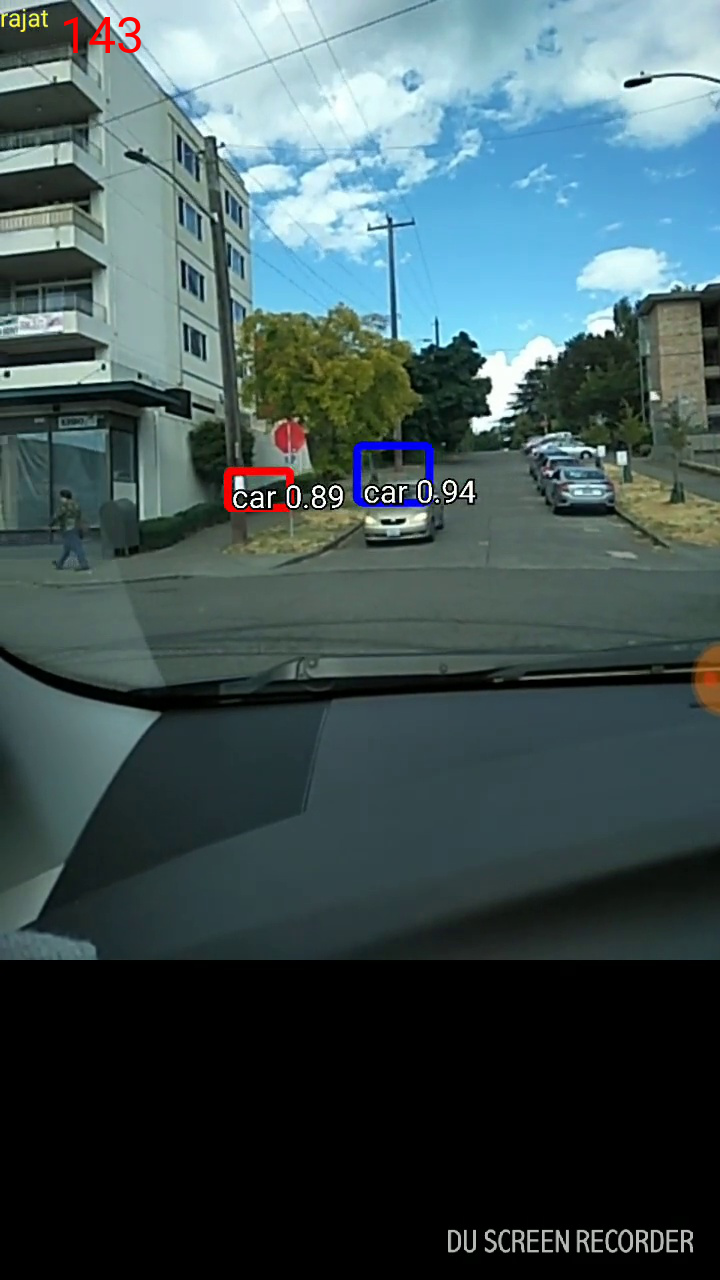
\includegraphics[width=\linewidth]{results/result_5720.png}
	\end{subfigure}
	\begin{subfigure}[b]{0.15\textwidth}
		\centering
		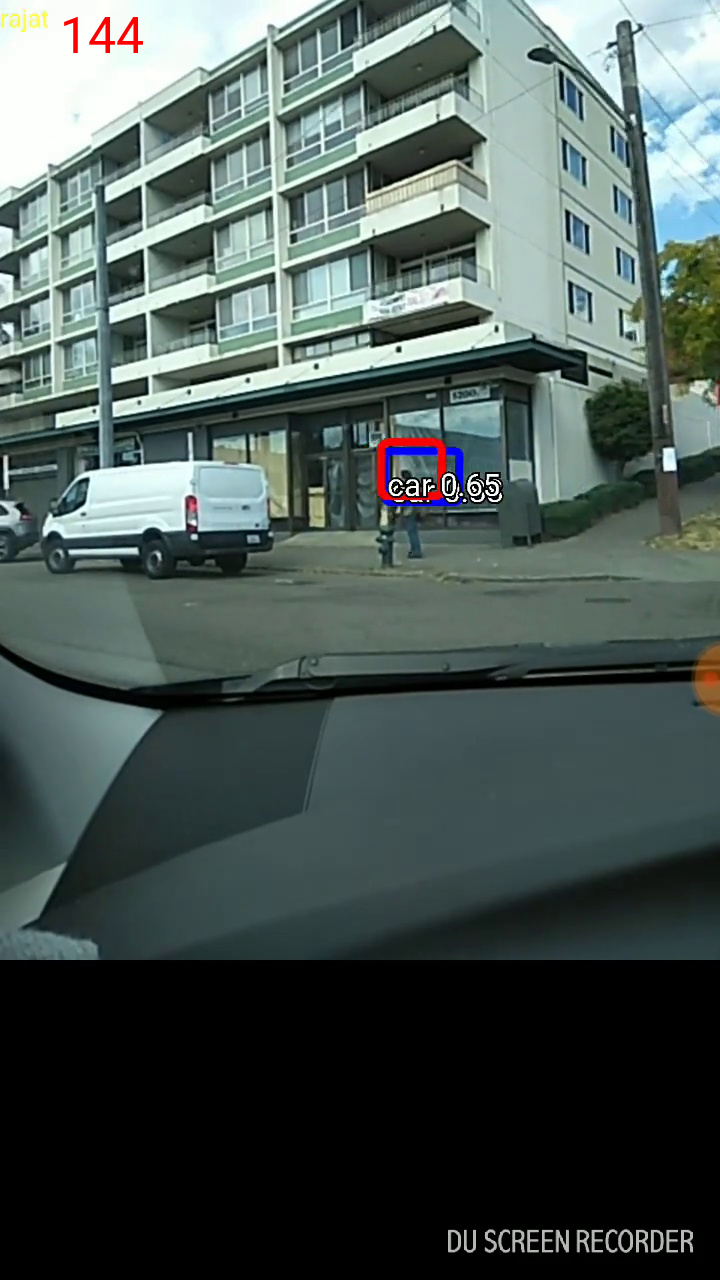
\includegraphics[width=\linewidth]{results/result_5760.png}
	\end{subfigure}
	\begin{subfigure}[b]{0.15\textwidth}
		\centering
		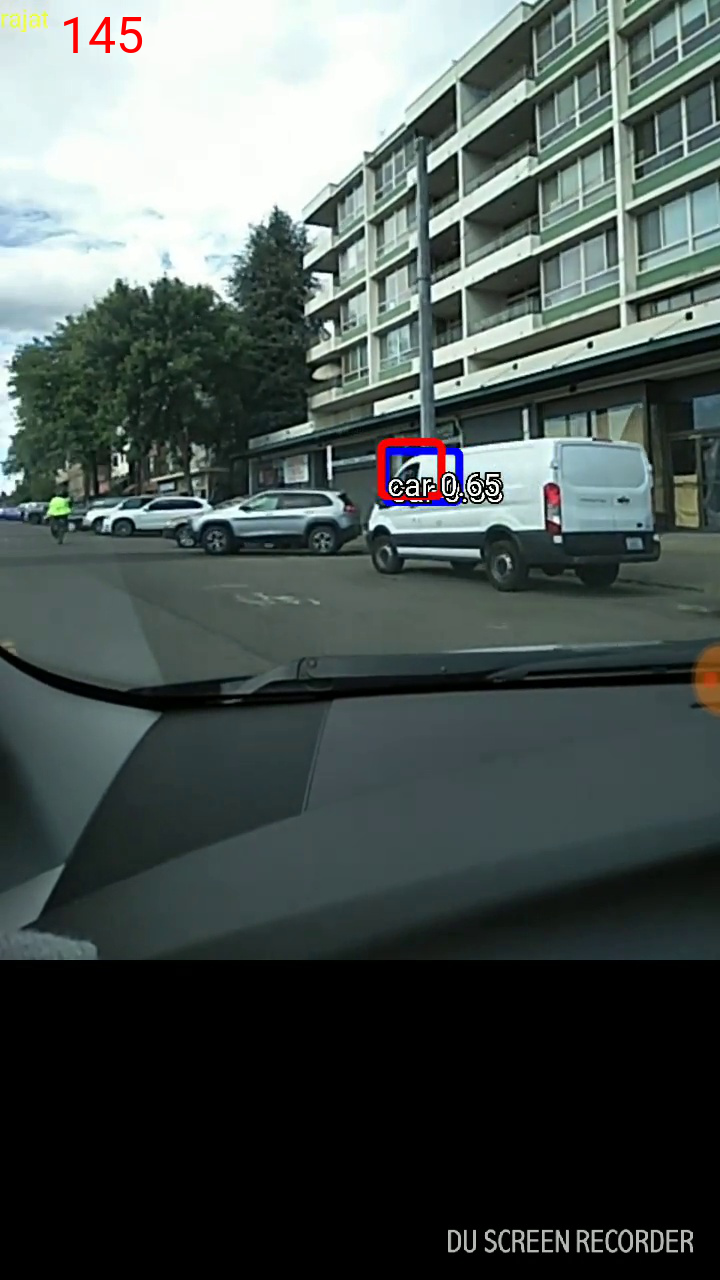
\includegraphics[width=\linewidth]{results/result_5800.png}
	\end{subfigure}
	\begin{subfigure}[b]{0.15\textwidth}
		\centering
		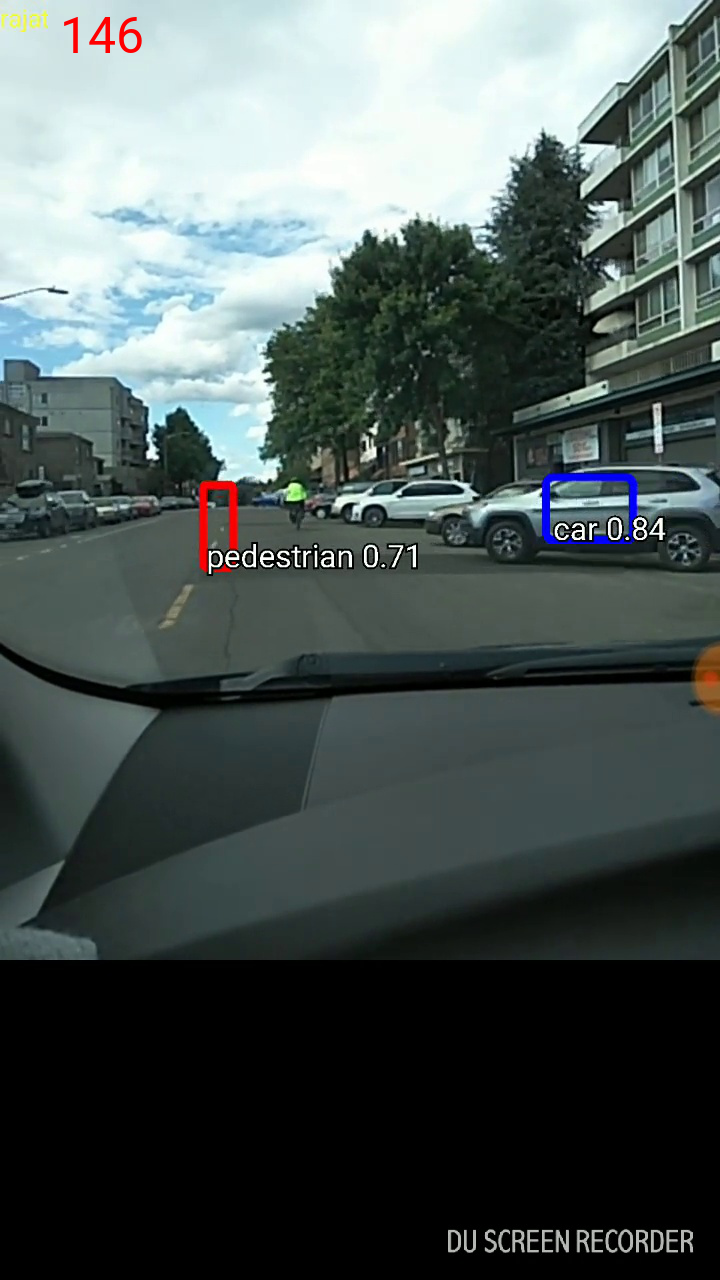
\includegraphics[width=\linewidth]{results/result_5840.png}
	\end{subfigure}
	\begin{subfigure}[b]{0.15\textwidth}
		\centering
		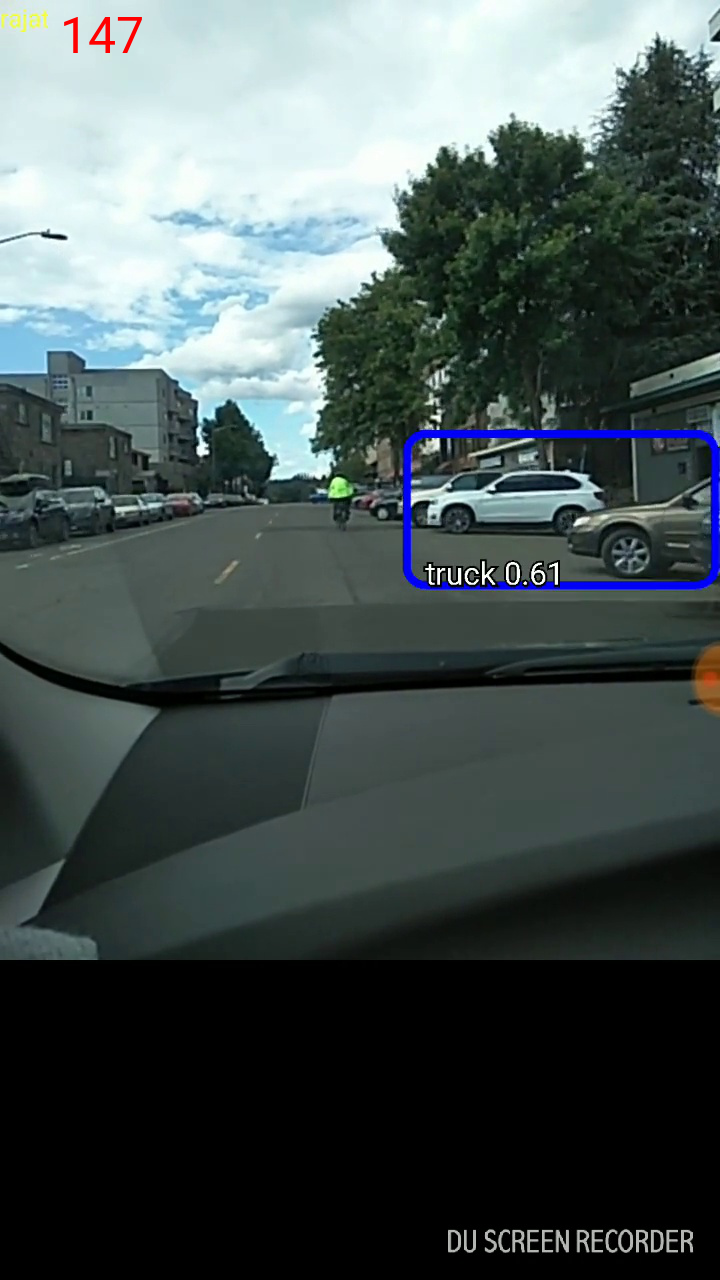
\includegraphics[width=\linewidth]{results/result_5880.png}
	\end{subfigure}
	\begin{subfigure}[b]{0.15\textwidth}
		\centering
		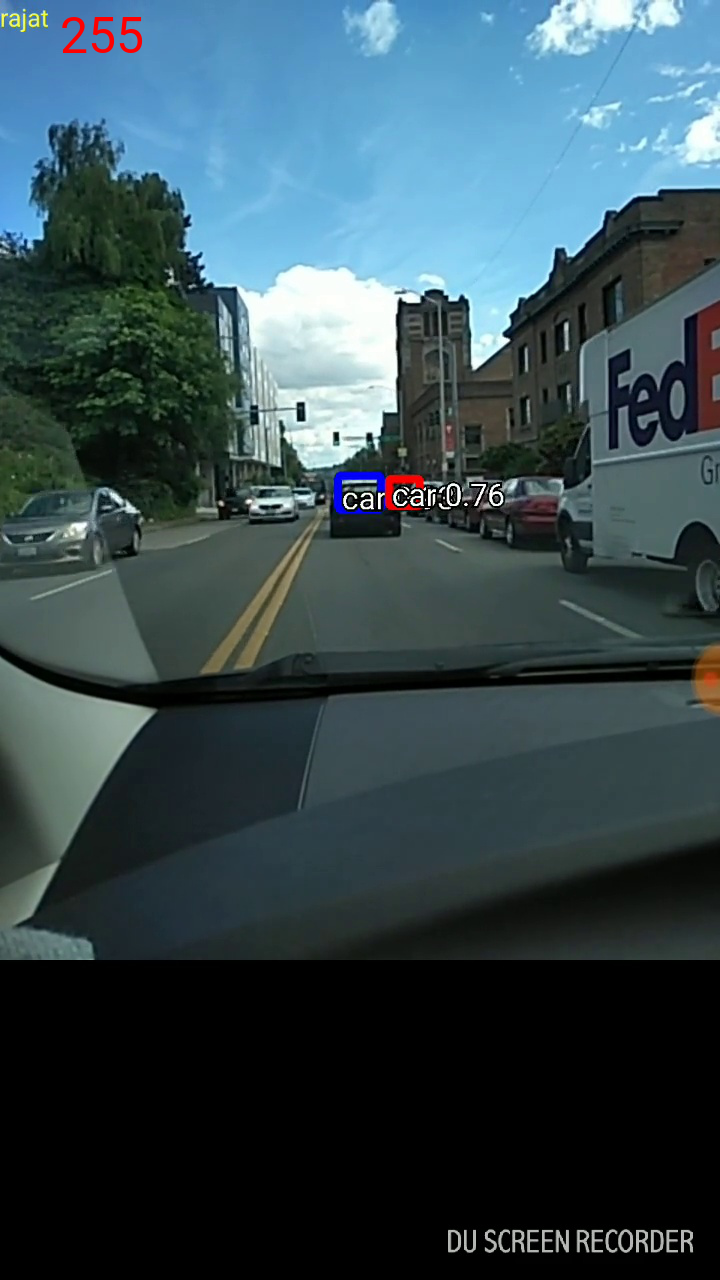
\includegraphics[width=\linewidth]{results/result_10200.png}
	\end{subfigure}
	\begin{subfigure}[b]{0.15\textwidth}
		\centering
		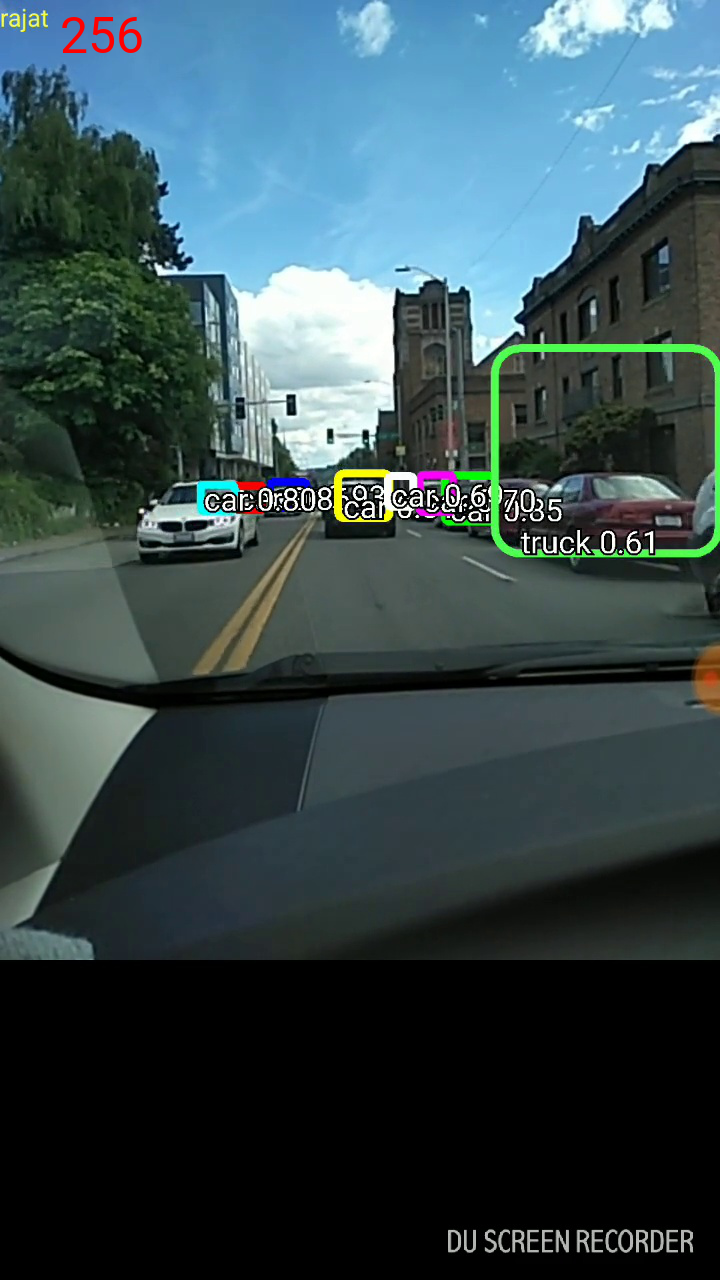
\includegraphics[width=\linewidth]{results/result_10240.png}
	\end{subfigure}
	\begin{subfigure}[b]{0.15\textwidth}
		\centering
		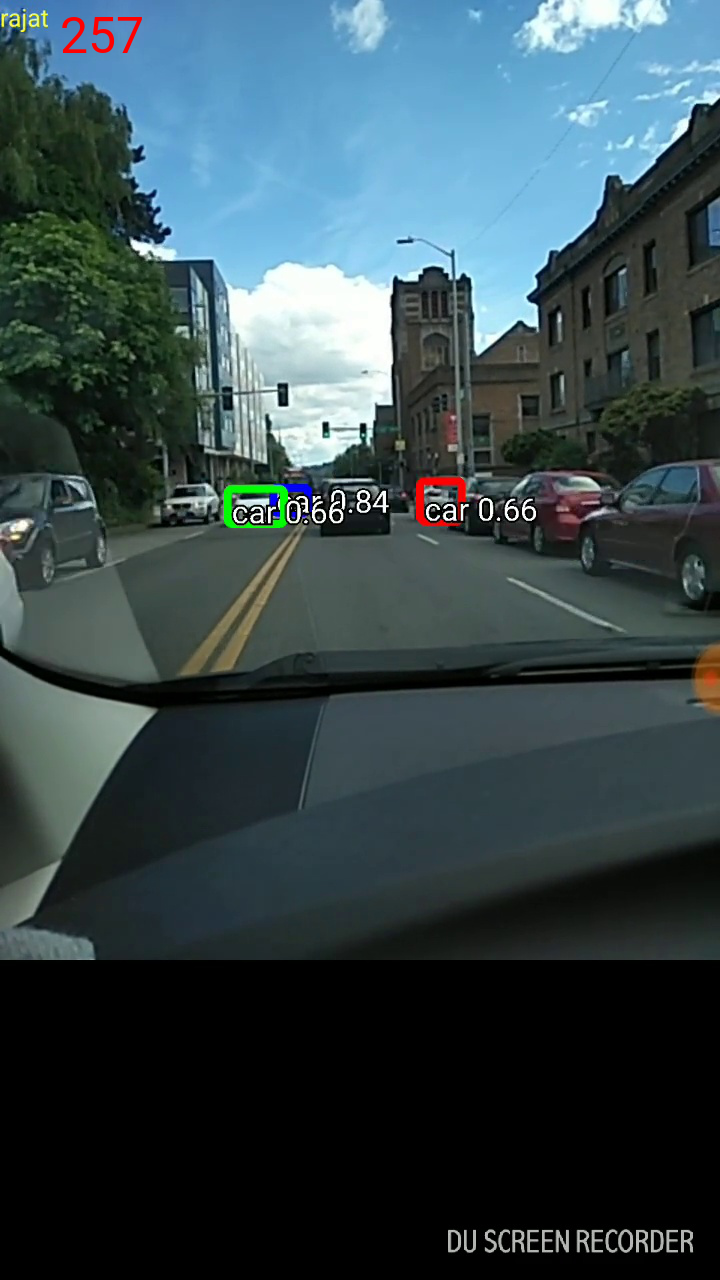
\includegraphics[width=\linewidth]{results/result_10280.png}
	\end{subfigure}
	\begin{subfigure}[b]{0.15\textwidth}
		\centering
		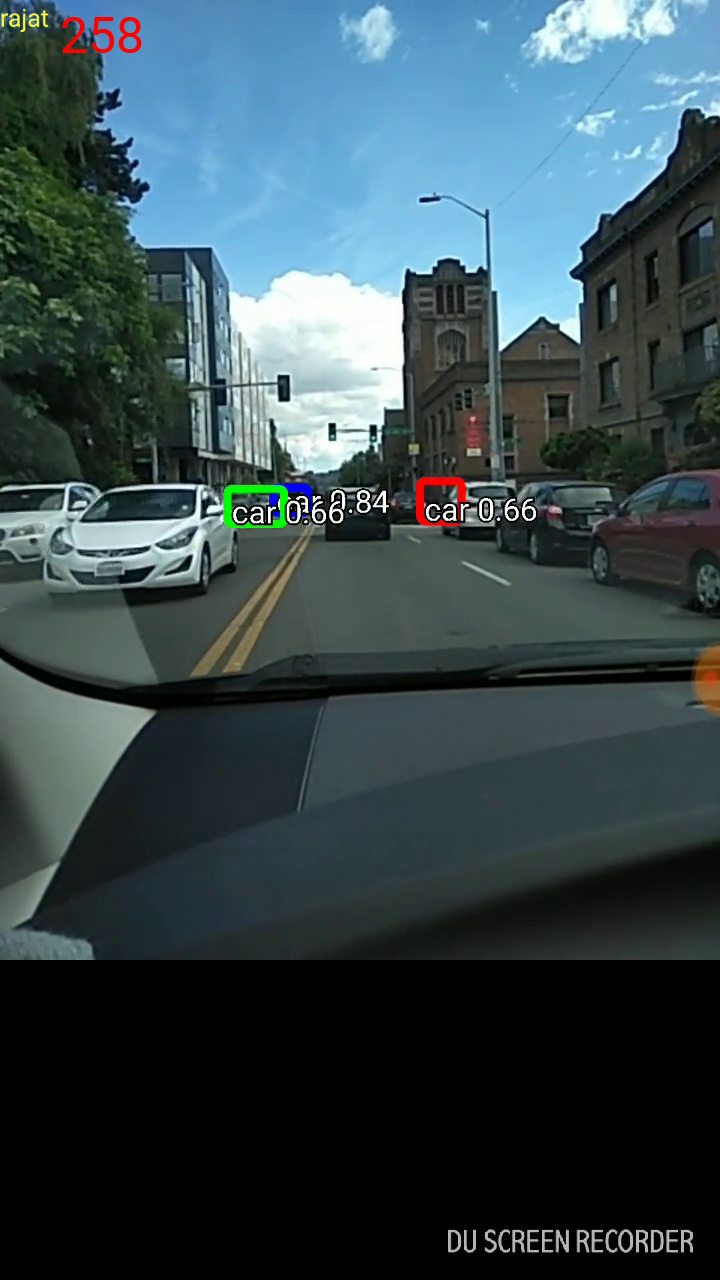
\includegraphics[width=\linewidth]{results/result_10320.png}
	\end{subfigure}
	\begin{subfigure}[b]{0.15\textwidth}
		\centering
		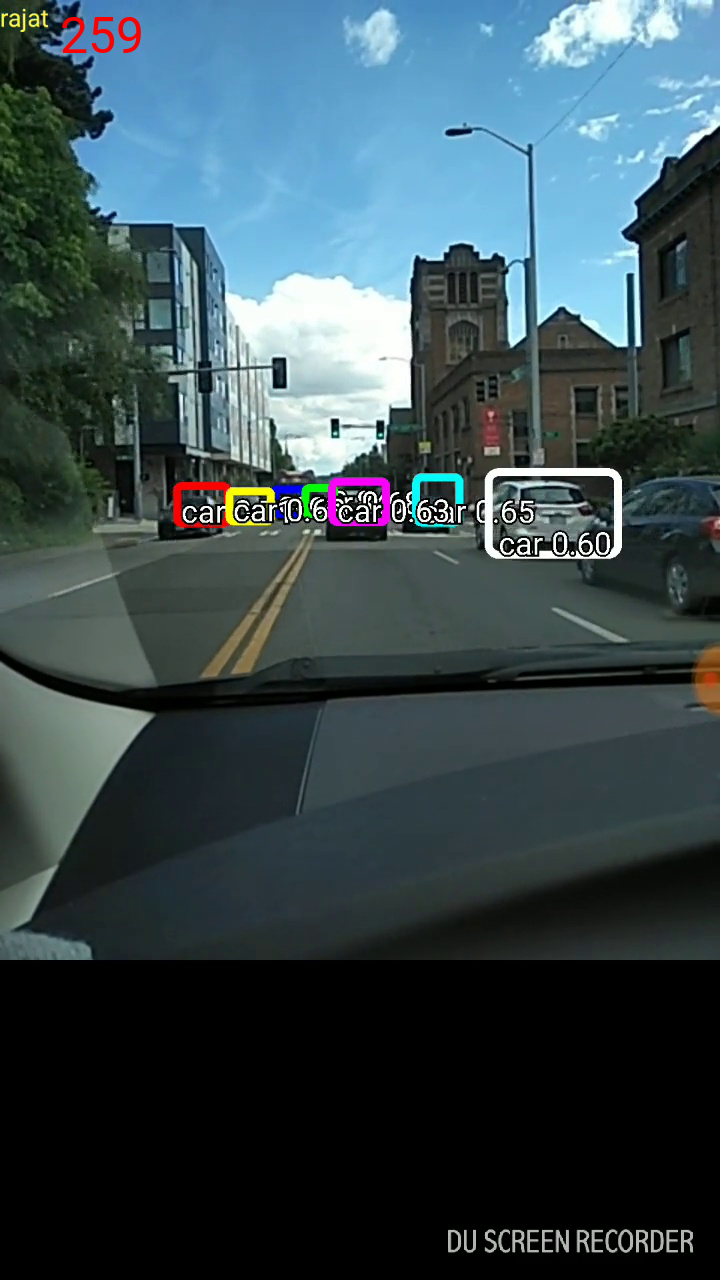
\includegraphics[width=\linewidth]{results/result_10360.png}
	\end{subfigure}
	\begin{subfigure}[b]{0.15\textwidth}
		\centering
		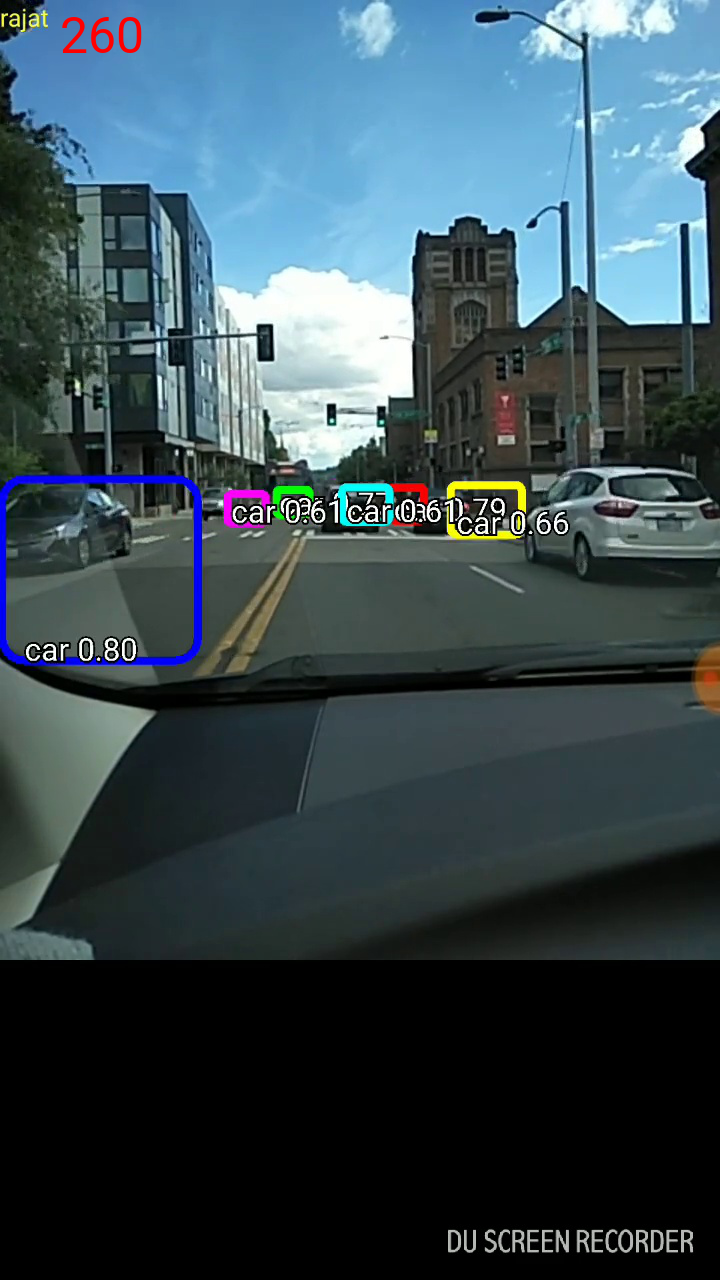
\includegraphics[width=\linewidth]{results/result_10400.png}
	\end{subfigure}
	\caption{(a) Taking a turn (b) Driving past a truck}
\end{figure}


\begin{figure}[H]
	\centering
	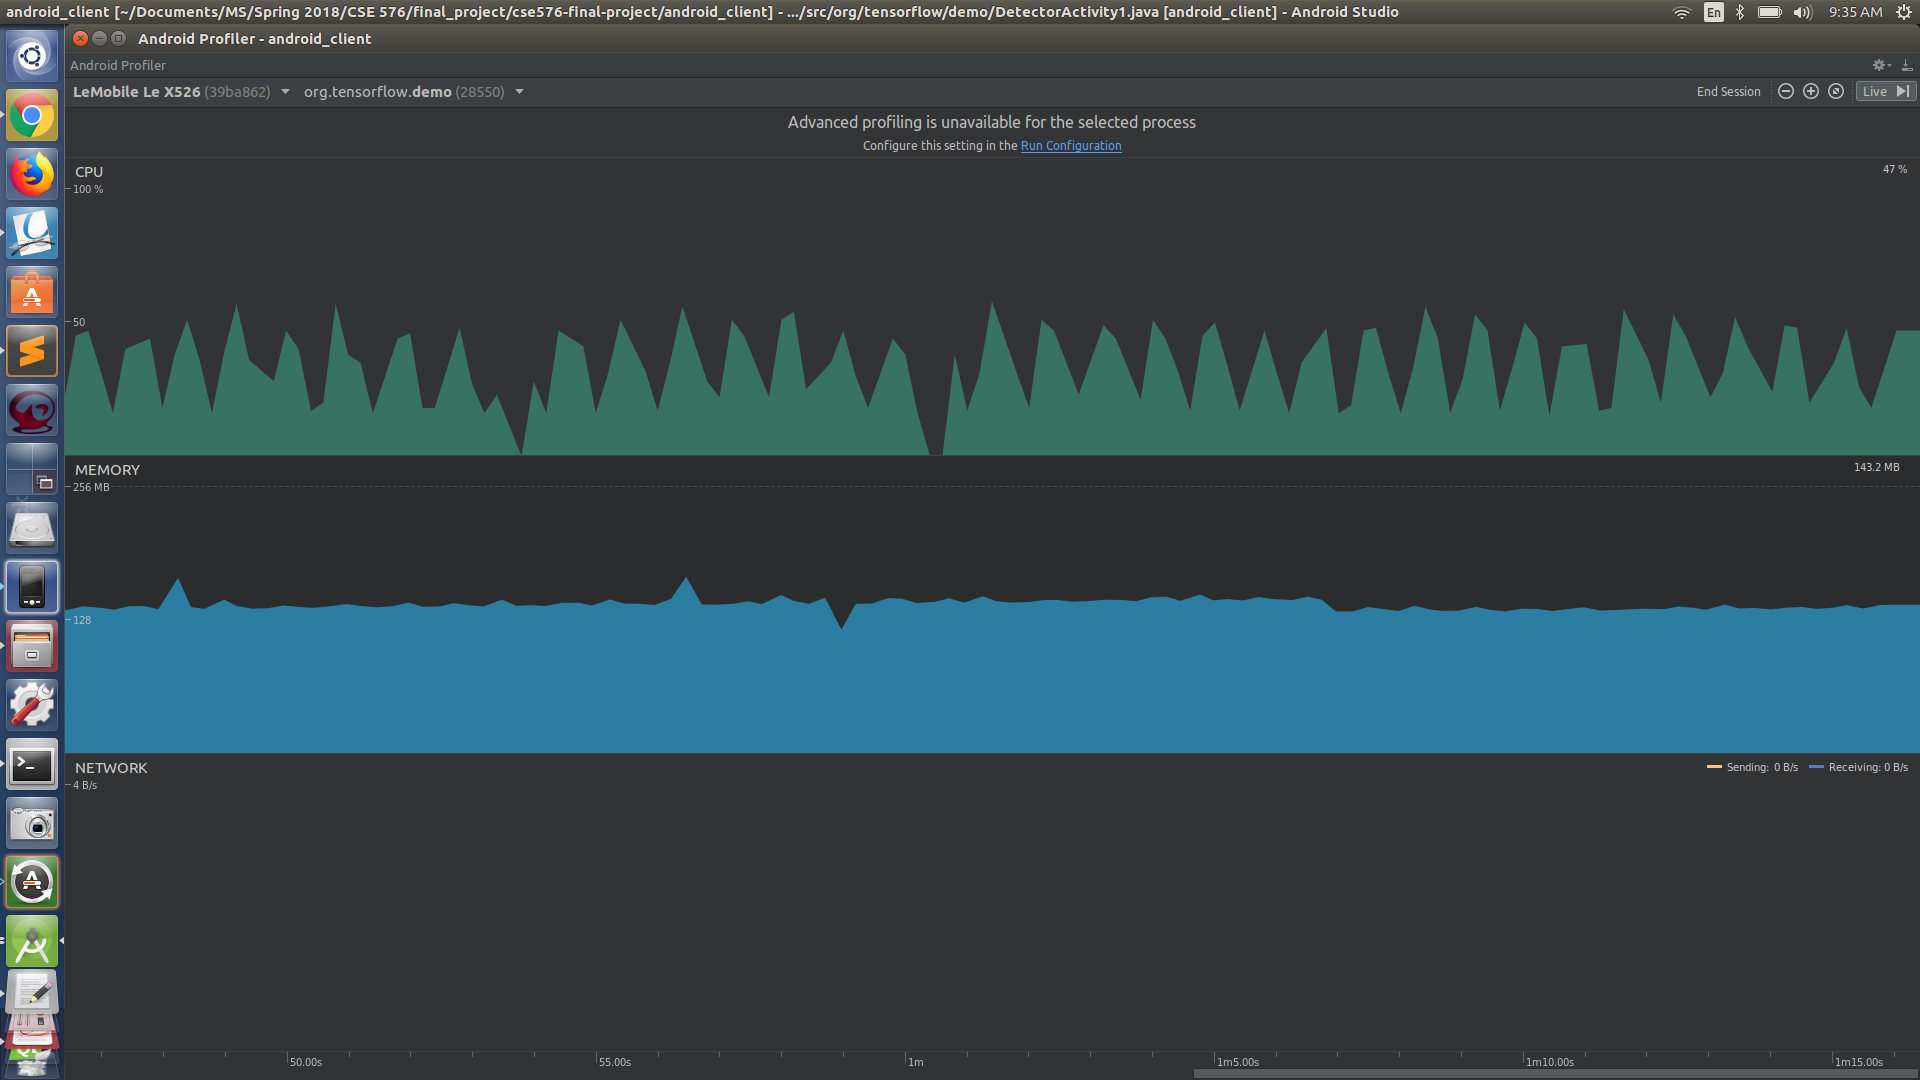
\includegraphics[width=0.75\linewidth]{performance.png}
	\caption{CPU and Memory usage while running the app}
\end{figure}

We used Android profiler to check the mobile's CPU and memory usage while the app was running. Figure 10 shows how the CPU usage bumps up every time the input data travels through the neural network for inference. It seems to be operating at 6-7 FPS which is four times less than the real time speed of 24 FPS. However we are are running this on the mobile's CPU and there is a scope for improvement in the future by exploting the device's GPU. Also the app just seems to use only 50\% of the cpu and we could further improve performance by incorporating parallelization in our android java code.  Moreover there are other mobile devices around with faster cpus and more RAM which could help increase the app's FPS and hence performance. 

\section{Conclusion}

In this project we used transfer learning to finetune a COCO pre-trained Mobilenet-SSD detector to adapt to the KITTI dataset. The trained model was evaluated according to VOC's evaluation criteria and then exported to run on Android mobile device using Tensorflow Android Interface Inference libraries. This project indicates the possibility of using a smartphone locally and independtly for object detection in autonomous driving. It outlines the necessary steps and concepts required all the way from training an object detection model to deploying it on mobile for autonomous navigation. The opportunities and challeneges mentioned here can serve as a steeping stone to future mobile based object detection applications. 


The project's Bitbucket repository can be found \href{https://bitbucket.org/rajatsc/cse576-final-project/src/master/}{here}.

\medskip

\bibliographystyle{plain}
\bibliography{refs_cv}

\end{document}
